%
\documentclass[12pt]{article}
% Oct 26, 1999
\setlength{\oddsidemargin}{-0.125in}
\setlength{\topmargin}{-0.5in} \setlength{\textwidth}{6.5in}
\setlength{\textheight}{9in}

\setlength{\textheight}{9in} \setlength{\textwidth}{6.5in}
\setlength{\topmargin}{-40pt} \setlength{\oddsidemargin}{0pt}
\setlength{\evensidemargin}{0pt}

\setlength{\textheight}{8.5in} \setlength{\textwidth}{6.5in}
\setlength{\topmargin}{-36pt} \setlength{\oddsidemargin}{0pt}
\setlength{\evensidemargin}{0pt} \tolerance=500
\renewcommand{\baselinestretch}{1.5}

\usepackage{amssymb, amsmath, latexsym, array, morefloats, epsfig, rotating, graphicx}
\usepackage{subfigure, url, mathtools, enumerate, wasysym, threeparttable, lscape}
\usepackage{natbib,color}
\usepackage{bm, bbm,epstopdf}
\usepackage{tikz}
\newcount\mycount
\usepackage{xr, zref, hyperref}

\newenvironment{proof}[1][Proof]{\begin{trivlist}
\item[\hskip \labelsep {\bfseries #1}]}{\end{trivlist}}
\newenvironment{definition}[1][Definition]{\begin{trivlist}
\item[\hskip \labelsep {\bfseries #1}]}{\end{trivlist}}
\newenvironment{example}[1][Example]{\begin{trivlist}
\item[\hskip \labelsep {\bfseries #1}]}{\end{trivlist}}
\newenvironment{remark}[1][Remark]{\begin{trivlist}
\item[\hskip \labelsep {\bfseries #1}]}{\end{trivlist}}

\newcommand{\qed}{\nobreak \ifvmode \relax \else
      \ifdim\lastskip<1.5em \hskip-\lastskip
      \hskip1.5em plus0em minus0.5em \fi \nobreak
      \vrule height0.75em width0.5em depth0.25em\fi}

%- Makes the section title start with Appendix in the appendix environment
 \newcommand{\Appendix}
 {%\appendix
 \def\thesection{\Alph{section}}
 \def\thesubsection{\Alph{section}.\arabic{subsection}}
 \def\theequation{\Alph{section}.\arabic{equation}}
 \def\thefigure{\Alph{section}.\arabic{figure}}
 \def\thealg{\Alph{section}.\arabic{alg}}
 %\def\thesubsection{A.\arabic{subsection}}
 }

\DeclareMathOperator{\vect}{vec}
\DeclareMathOperator{\vech}{vech}
\DeclareMathOperator{\diag}{diag}

\newtheorem{alg}{Algorithm}

% if variable blind is undefined, assume it is 0
\makeatletter
\@ifundefined{blind}{\def\blind{0}}{}
\makeatother

% if not blinded, reference unblinded paper
\if0\blind
{
  \externaldocument{psostat}
}\fi

% if blinded, reference blinded paper
\if1\blind
{
  \externaldocument{psostatblind}
}\fi


%%%%%%%%%%%%%%%%%%%%%%%%%%%%%%%%%%%%%
\begin{document}
\thispagestyle{empty} \baselineskip=28pt

\thispagestyle{empty} \baselineskip=28pt

%
\begin{center}
%{\LARGE{\bf Supplemental Web Material: Particle Swarm Optimization Assisted Metropolis Hastings Algorithms}}
{\LARGE{\bf Particle Swarm Optimization Assisted Metropolis Hastings Algorithms}}
\end{center}


\baselineskip=12pt


%%
%%
%%
%%%%%%%%%%%%%%%%%%%%%%%%%%%%%%%%%%%%%%%%%%%%%%%%%%%%%%%%%%%%%%%%%%%%%%%%

\vskip 2mm
% if not blinded, list the authors on the title page
\if0\blind
{
  \begin{center}
    Matthew Simpson,\footnote{(\baselineskip=10pt to whom correspondence should be addressed)
      Department of Statistics, University of Missouri,
      146 Middlebush Hall, Columbia, MO 65211-6100, themattsimpson@gmail.com}
    % Christopher K. Wikle,\footnote{\label{note:aff}\baselineskip=10pt
    % Department of Statistics, University of Missouri,
    % 146 Middlebush Hall, Columbia, MO 65211-6100}
    % and Scott H. Holan\textsuperscript{\ref{note:aff}}
  \end{center}
} \fi

\clearpage\pagebreak\newpage \pagenumbering{arabic}

\baselineskip=24pt

\Appendix
\section{PSO and BBPSO details}\label{app:psodetail}

In Section \ref{sec:pso} we introduced PSO, BBPSO, and our adaptively tuned variants of both. Here we describe in detail several BBPSO variants as well as a class of neighborhood topologies called the ring topologies.

\subsection{BBPSO}\label{subapp:bbpso}
The standard BBPSO algorithm was introduced by \citet{kennedy2003bare} and updates from $t$ to $t+1$ via equation \eqref{eq:bbpso}. A commonly used variant of BBPSO also introduced by \citet{kennedy2003bare} is called BBPSOxp. In this variant, each coordinate of each particle has a 50\% chance of updating according to \eqref{eq:bbpso} and a 50\% chance of moving directly to that particle's personal best location on that coordinate. In other words
\begin{align}\label{eq:bbpsoxp}
\theta_{ij}(t+1) = \begin{cases} N\left(\frac{p_{ij}(t) + g_{ij}(t)}{2}, s^2_{ij}(t)\right) & \mbox{with probability }0.5\\
p_{ij}(t) &\mbox{otherwise,}\end{cases}
\end{align}
where $s_{ij}(t) = |p_{ij}(t) - g_{ij}(t)|$.

A downside of both BBPSO and BBPSOxp is that any particle whose personal best is currently its group best location does not move due to the definition of the standard deviation term. Several methods have been proposed to overcome this; e.g. \citet{hsieh2010modified} and \citet{zhang2011novel}. \citet{zhang2011novel} propose using mutation and crossover operations for the group best particle. To do this, each group best particle randomly selects three other distinct particles from the entire swarm, $i_1$, $i_2$, and $i_3$, and updates according to
\begin{align}\label{eq:bbpsomc}
\theta_{ij}(t+1) = p_{i_1j}(t) + 0.5\{p_{i_2j}(t) - p_{i_3j}(t)\}.
\end{align}
This combines easily with BBPSOxp to create BBPSOxp-MC by updating group best particles according to \eqref{eq:bbpsomc} and all other particles according to \eqref{eq:bbpsoxp}, but it does not completely solve the problem in BBPSOxp-MC. A particle which finds a personal best that is the same as its group best on some but not all coordinates due to the ``xp'' component of BBPSOxp-MC will have a standard deviation of zero for those coordinates during the next iteration. This is easily overcome by using the ``MC'' operation for those coordinates as well. So both BBPSOxp-MC and BBPSO-MC can be encapsulated into the following general BBPSO algorithm. For each particle $i$, sample three other particles $i_1$, $i_2$, $i_3$ from the swarm, and for each coordinate $j$ let $s_{ij}(t) = |p_{ij}(t) - g_{ij}(t)|$. Then the general updating equation is
\begin{align}\label{eq:bbpsoall}
\theta_{ij}(t+1) = 
  \begin{cases} 
    \begin{cases} N\left(\frac{p_{ij}(t) + g_{ij}(t)}{2}, s^2_{ij}(t)\right) & \mbox{with probability } \rho\\
      p_{ij}(t) & \mbox{with probability } 1 - \rho,
    \end{cases}
    & \mbox{ if } s^2_{ij}(t) > 0\\
    p_{i_1j}(t) + 0.5\{p_{i_2j}(t) - p_{i_3j}(t)\} & \mbox{ otherwise.}
  \end{cases}
\end{align}
When $\rho = 0$ we have BBPSO-MC, and when $\rho = 0.5$ we have BBPSOxp-MC. These are the two BBPSO variants that we consider.

Similarly, we can create adaptively tuned versions of BBPSO-MC and BBPSOxp-MC by analogy with \eqref{eq:at-bbpso} and \eqref{eq:bbpsoall}:
\begin{align*}%\label{eq:at-bbpsoall}
\theta_{ij}(t+1) &= 
  \begin{cases} 
    \begin{cases} t_{df}\left(\frac{p_{ij}(t) + g_{ij}(t)}{2}, \sigma^2(t)s^2_{ij}(t)\right) & \mbox{with probability } \rho\\
      p_{ij}(t) & \mbox{with probability } 1 - \rho,
    \end{cases}
    & \mbox{ if } s^2_{ij}(t) > 0\\
    p_{i_1j}(t) + 0.5\{p_{i_2j}(t) - p_{i_3j}(t)\} & \mbox{ otherwise.}
  \end{cases}\\
\log\sigma^2(t+1) &= \log\sigma^2(t) + c\times\{R(t+1) - R^*\},
\end{align*}
where $R(t)=\#\{i:Q(\bm{p}_i(t))> Q(\bm{p}_i(t-1))\}/n$, and $df$, $R^*$, and $c$ are defined in Section \ref{subsec:ATBBPSO}. Then AT-BBPSO-MC sets $\rho=0$ and AT-BBPSOxp-MC sets $\rho=0.5$.

\subsection{Ring-$k$ neighborhood topologies}\label{subapp:ring}
For all PSO and BBPSO algorithms, the group best location for a given particle is defined relative to the particle's group. To wit $\bm{g}_i(t+1) = \arg\max_{\{\bm{p}_j(t+1)|j\in\mathcal{N}_i\}}Q(\bm{p}_j(t+1))$ where $\mathcal{N}_i$ is the set of particles that part of particle $i$'s group, or are ``neighbors'' of particle $i$. The default neighborhood topology is $\mathcal{N}_i = \{1, 2, \dots, n\}$ where $n$ is the number of particles, so each particle is in each other particle's neighborhood. PSO and BBPSO algorithms using this topology are often call gbest swarms or gbest algorithms. 

The main problem with gbest PSO and BBPSO algorithms is that by allowing each particle to see the best location of the entire swarm, they curtail early exploration of the search space. In order to restrict the flow of information across the swarm and allow for more exploration, it is often useful to only allow each particle to see a subset of the other particles using a more restrictive neighborhood topology. There are several commonly used neighborhood topologies [CITATION], but we will use the ring topologies. The ring-$k$ neighborhood topology for $k=1,2,\dots,\lceil n/2\rceil$ is defined as follows. Arrange the particles in a circle, as in Figure \ref{fig:ring}. Then each particle is neighbors with the $k$ particles to its left and the $k$ particles to its right. That is, $\mathcal{N}_i = \{i-k, i-k+1, \dots, i-1, i+1, \dots, i+k-1, i+k\}$ where addition and subtraction are modulo $n$ so that e.g. $n + 1 = 1$. The value of $k$ controls how quickly information moves around the swarm --- the larger $k$, the faster it moves. In the limit of $k=\lceil n/2 \rceil$, we have the global neighborhood topology.

\begin{figure}
  \centering
  {
    \begin{tikzpicture}[transform shape]
      % the multiplication with floats is not possible. Thus I split the loop in two.
      \foreach \number in {1,...,7}{
        % Computer angle:
        \mycount=\number
        \advance\mycount by 2
        \multiply\mycount by 45
        \advance\mycount by 0
        \node[draw,circle,inner sep=0.1cm] (N-\number) at (\the\mycount:1cm) {};
      }
      \foreach \number in {10,...,15}{
        % Computer angle:
        \mycount=\number
        \advance\mycount by 1
        \multiply\mycount by 45
        \advance\mycount by 22.5
        \node[draw,circle,inner sep=0.1cm] (N-\number) at (\the\mycount:1cm) {};
      }
      \foreach \number in {1,...,2}{
        % Computer angle:
        \mycount=\number
        \advance\mycount by 0
        \multiply\mycount by 45
        \advance\mycount by 22.5
        \node[circle,inner sep=0.1cm,fill=gray] (N-\number) at (\the\mycount:1cm) {};
      }
      \foreach \number in {1,...,1}{
        % Computer angle:
        \mycount=\number
        \advance\mycount by 1
        \multiply\mycount by 45
        \advance\mycount by 0
        \node[draw=black,circle,inner sep=0.1cm,fill=black,label=Ring-1] (N-\number) at (\the\mycount:1cm) {};
      }
    \end{tikzpicture}
  }
  {
    \begin{tikzpicture}[transform shape]
      % the multiplication with floats is not possible. Thus I split the loop in two.
      \foreach \number in {2,...,6}{
        % Computer angle:
        \mycount=\number
        \advance\mycount by 2
        \multiply\mycount by 45
        \advance\mycount by 0
        \node[draw,circle,inner sep=0.1cm] (N-\number) at (\the\mycount:1cm) {};
      }
      \foreach \number in {10,...,15}{
        % Computer angle:
        \mycount=\number
        \advance\mycount by 1
        \multiply\mycount by 45
        \advance\mycount by 22.5
        \node[draw,circle,inner sep=0.1cm] (N-\number) at (\the\mycount:1cm) {};
      }
      \foreach \number in {1,...,2}{
        % Computer angle:
        \mycount=\number
        \advance\mycount by 0
        \multiply\mycount by 45
        \advance\mycount by 22.5
        \node[circle,inner sep=0.1cm,fill=gray] (N-\number) at (\the\mycount:1cm) {};
      }
      \foreach \number in {1,...,3}{
        % Computer angle:
        \mycount=\number
        \advance\mycount by 0
        \multiply\mycount by 45
        \advance\mycount by 0
        \node[circle,inner sep=0.1cm,fill=gray] (N-\number) at (\the\mycount:1cm) {};
      }
      \foreach \number in {1,...,1}{
        % Computer angle:
        \mycount=\number
        \advance\mycount by 1
        \multiply\mycount by 45
        \advance\mycount by 0
        \node[draw=black,circle,inner sep=0.1cm,fill=black,label=Ring-2] (N-\number) at (\the\mycount:1cm) {};
      }
    \end{tikzpicture}
  }
  {
    \begin{tikzpicture}[transform shape]
      % the multiplication with floats is not possible. Thus I split the loop in two.
      \foreach \number in {2,...,6}{
        % Computer angle:
        \mycount=\number
        \advance\mycount by 2
        \multiply\mycount by 45
        \advance\mycount by 0
        \node[draw,circle,inner sep=0.1cm] (N-\number) at (\the\mycount:1cm) {};
      }
      \foreach \number in {10,...,15}{
        % Computer angle:
        \mycount=\number
        \advance\mycount by 1
        \multiply\mycount by 45
        \advance\mycount by 22.5
        \node[draw,circle,inner sep=0.1cm] (N-\number) at (\the\mycount:1cm) {};
      }
      \foreach \number in {1,...,4}{
        % Computer angle:
        \mycount=\number
        \advance\mycount by -1
        \multiply\mycount by 45
        \advance\mycount by 22.5
        \node[circle,inner sep=0.1cm,fill=gray] (N-\number) at (\the\mycount:1cm) {};
      }
      \foreach \number in {1,...,3}{
        % Computer angle:
        \mycount=\number
        \advance\mycount by 0
        \multiply\mycount by 45
        \advance\mycount by 0
        \node[circle,inner sep=0.1cm,fill=gray] (N-\number) at (\the\mycount:1cm) {};
      }
      \foreach \number in {1,...,1}{
        % Computer angle:
        \mycount=\number
        \advance\mycount by 1
        \multiply\mycount by 45
        \advance\mycount by 0
        \node[draw=black,circle,inner sep=0.1cm,fill=black,label=Ring-3] (N-\number) at (\the\mycount:1cm) {};
      }
    \end{tikzpicture}
  }
  {
    \begin{tikzpicture}[transform shape]
      % the multiplication with floats is not possible. Thus I split the loop in two.
      \foreach \number in {2,...,8}{
        % Computer angle:
        \mycount=\number
        \advance\mycount by 1
        \multiply\mycount by 45
        \advance\mycount by 0
        \node[draw,circle,inner sep=0.1cm,fill=gray] (N-\number) at (\the\mycount:1cm) {};
      }
      \foreach \number in {9,...,16}{
        % Computer angle:
        \mycount=\number
        \advance\mycount by 1
        \multiply\mycount by 45
        \advance\mycount by 22.5
        \node[draw,circle,inner sep=0.1cm,fill=gray] (N-\number) at (\the\mycount:1cm) {};
      }
      \foreach \number in {1,...,1}{
        % Computer angle:
        \mycount=\number
        \advance\mycount by 1
        \multiply\mycount by 45
        \advance\mycount by 0
        \node[draw=black,circle,inner sep=0.1cm,fill=black,label=Global] (N-\number) at (\the\mycount:1cm) {};
      }
    \end{tikzpicture}
  }
  \caption{Ring-$k$ and global neighborhood topologies. Filled in gray particles are neighbors of the filled in black particle.}
  \label{fig:ring}
\end{figure}



\section{Comparing PSO and BBPSO algorithms}\label{app:psocompare}
In order to compare AT-BBPSO to other PSO variants, we employ a subset of test functions used in \citet{hsieh2010modified}. Each function is listed in Table \ref{tab:testfuns} along with the global maximum and argmax, and the initialization range for the simulations. Further description of many of these functions can be found in \citet{clerc2010particle}. For each function, we set $D=20$ so the domain of each function is $\Re^{20}$. For each function, the PSO algorithms are initialized in a range that does not contain the true maximum.

\begin{table}[h]
\centering
\begin{tabular}{llll}
 Equation & ArgMax & Maximum & Initialization \\\hline
 $Q_1(\bm{\theta}) = -\sum_{i=1}^D\theta_i^2$ & $\bm{\theta}^* = \bm{0}$ & $Q_1(\bm{\theta}^*) = 0$  & $(50, 100)^D$ \\
 $Q_2(\bm{\theta}) = -\sum_{i=1}^D\left(\sum_{j=1}^i \theta_j\right)^2 $ & $\bm{\theta}^* = \bm{0}$ & $Q_2(\bm{\theta}^*) = 0$ & $(50, 100)^D$ \\
% $Q_3(\bm{\theta}) = -0.5 - \frac{\sin(||\bm{\theta}||) - 0.5}{\left(1 + 0.001||\bm{\theta}||^2\right)^2}$ & $\left\{||\bm{\theta}^*|| \approx 4.6849\right\}$ & $Q_3(\bm{\theta}^*) \approx 0.9358$ & $(50, 100)^D$ \\ 
 $Q_3(\bm{\theta}) = -\sum_{i=1}^{D-1}\left[100\{\theta_{i+1} + 1 - (\theta_i + 1)^2\} + \theta_i^2\right]$ & $\bm{\theta}^* = \bm{0}$ & $Q_3(\bm{\theta}^*) = 0$ & $(15, 30)^D$ \\
 $Q_4(\bm{\theta}) = 9D - \sum_{i=1}^D\{\theta_i^2 - \cos(2\pi \theta_i) + 10\}$ & $\bm{\theta}^*=\bm{0}$ & $Q_4(\bm{\theta}^*) = 0$ & $(2.56, 5.12)^D$ \\
 %$Q_6(\bm{\theta}) = \sum_{i=1}^D\theta_i\sin\left(\sqrt{|\theta_i|}\right)$ & None & None & $(-500, -250)^D$ \\
 $Q_5(\bm{\theta}) = -\frac{1}{4000}||\bm{\theta}||^2 + \prod_{i=1}^D\cos\left(\frac{\theta_i}{\sqrt{i}}\right) - 1$ & $\bm{\theta}^* = \bm{0}$ & $Q_5(\bm{\theta}^*) = 0$ & $(300, 600)^D$ \\
 \shortstack[l]{$Q_6(\bm{\theta}) = 20\exp\left(-0.2\sqrt{\frac{1}{D}||\bm{\theta}||}\right)$ \\ \ \ \ \ \ \ \ \ $+ \exp\left\{\frac{1}{D}\sum_{i=1}^D\cos(2\pi \theta_i)\right\} - 20 - \exp(1)$} & $\bm{\theta}^* = \bm{0}$ & $Q_6(\bm{\theta}^*) = 0$ & $(16, 32)^D$\\\hline
\end{tabular}
\caption{Test functions for evaluating PSO algorithms. The dimension of $\bm{\theta}$ is $D$ and $||.||$ is the Euclidean norm: $||\bm{\theta}|| = \sqrt{\sum_{i=1}^D\theta_i^2}$.} 
\label{tab:testfuns}
\end{table}

We use several PSO algorithms in the simulation study. The standard PSO algorithm uses the parameter values suggested by \cite{blum2008swarm} and \cite{clerc2002particle}. The AT-BBPSO variants are implemented a wide variety of parameter values, but all have the scale parameter initialized at $\sigma(0)=1$, and both set $c=0.1$. The AT-PSO variants are initialized at $\omega(0)=1$ and also set $c=0.1$. In addition, each algorithm is implemented using each of three neighborhood structures --- the global, ring-3, and ring-1 neighborhoods. Each algorithm was used to optimize each objective function for 500 iterations over 50 replications using 20 particles. Initializations were changed across replications but held constant across algorithms. The standard PSO, DI-PSO, and AT-PSO algorithms initialized their velocity terms using the same method as a function of the initial locations of the particles, which we will denote by $\bm{x}_i$ for particle $i$. Let $x_{max,j}$ be the maximum initial value of coordinate $j$ of $\bm{x}_i$ for each particle $i$, and let $x_{min,j}$ be the corresponding minimum. Then let $d_{max} = max_{j}x_{max,j} - x_{min,j}$. Then we initialize the velocities with $v_{ij}(0)\stackrel{iid}{\sim}U(-d_{max}/2,d_{max}/2)$. Tables \ref{tab:psosim1}-\ref{tab:psosim6} contain the simulation results for objective functions 1-6 respectively (OF1, OF2, etc.). We use several measures to quantify how well each algorithm finds the global maximum. First, each table includes the mean and standard deviation of the absolute difference between the true global maximum and the algorithm's estimated global maximum across all 50 replications, denoted by Mean and SD. Second, each table includes a convergence criterion --- the proportion of the replications that came within $0.01$ of the true global maximum, denoted by $\widehat{p}$. Finally, $\widehat{t}$ denotes the median number of iterations until the algorithm reaches the convergence criterion. When $\hat{p}<0.5$ then $\hat{t} = \infty$ since greater than 50\% of the replications did not converge in the maximum number of iterations allowed. Then Mean, $\hat{p}$, and $\hat{t}$ can be thought of how close the algorithm gets to the global maximum on average, what proportion of the time it converges, and long it takes to converge respectively.

We highlight only some of the features of these tables. First and foremost, PSO, BBPSO-MC, and BBPSOxp-MC almost always do worse than their AT cousins. Adaptively tuning either the scale or inertia parameter leads to gains in all three of our measures, sometimes large. The comparison is starkest between BBPSO variants and AT-BBPSO variants, partially because BBPSO tends to be pretty bad but also because AT-BBPSO does very well. Second, for most non-AT algorithms the more restrictive neighborhoods appear to yield algorithms which do a better job of finding the global max. For the AT-PSO algorithms, it appears that the target improvement rate ($R^*$) and the neighborhood interact. When the rate is high a more restrictive neighborhood is preferable, while when the rate is low a less restrictive neighborhood is preferable. On the other hand, for the AT-BBPSO algorithms, the opposite appears to be true --- when the target improvement rate is high, a less restrictive neighborhood is desirable and vice versa. In addition, the best AT-BBPSO algorithms often use the global neighborhood while for the other classes of algorithms their best versions typically use the ring-1 or ring-3 neighborhood.

For the DI-PSO algorithms often there is a parameter-neighborhood combination that does well, typically from setting $\alpha=200$ (20\% of the 500 iterations) and $\beta=1$ and using either the ring-1 or ring-3 neighborhood. One of these combinations typically does the best of all the DI-PSO algorithms but they can sometimes still do much worse than the best alternatives (e.g., for OF2). In the AT-BBPSO algorithms, it is not always clear what the best parameter settings are, but good default values appear to be $df=3$ or $5$ and $R^*=0.3$ or $0.5$. When these values are good, they often lead to the best performing PSO algorithms we consider. However, it is not always clear whether to use AT-BBPSO-MC or AT-BBPSOxp-MC. For some objective functions, e.g. OF4, the xp version is consistently better than the non-xp alternative, but the opposite is true for others, e.g. OF2.. AT-PSO is also often very competitive with $R^*=0.3$ or $R^*=0.5$, though again sometimes different parameter settings also appear to work well. 

The DI-PSO and AT-PSO algorithms are similar conceptually, but often yield very different results. DI-PSO deterministically reduces the inertia parameter over time in the same manner given a fixed set of parameter values ($\alpha$ and $\beta$), while AT-PSO dynamically adjusts the inertia parameter to hit a target improvement rate. Figure \ref{fig:inertia} plots the inertia over time for the DI-PSO algorithm with $\alpha=200$ and $\beta=1$, and observed inertia over time for one replication of the AT-PSO algorithm with target rate $R^*=0.5$ and ring-1 neighborhood for OF1 and one replication for OF6. All three algorithms have an initial inertia of $\omega(0)=1$. While DI-PSO smoothly decreases its inertia with a slowly decreasing rate, AT-PSO very quickly drops its inertia for OF1 to about 0.55 then bounces around around near that point. It also jumps up above 1 initially, imploring the particles to cast a wider net in search of higher value areas of the search space. This is pretty typical behavior for the inertia parameter of AT-PSO --- it tends to bounce around a level which is approximately the average over time of the DI-PSO's inertia, though lower values of $R^*$ will result in higher inertias. In this way, AT-PSO alternates periods of exploration (relatively high inertia) and periods of exploitation (relatively low inertia). The main exception to this pattern is when AT-PSO converges around a local maximum. In this case, inertia plummets to zero as the particles settle down. This is precisely what happens for OF6 in Figure \ref{fig:inertia}, though in this case the maximum is not global --- Table \ref{tab:psosim6} indicates that ring-1 AT-PSO with $R^*=0.5$ never converged to the global max. In optimization problems with multiple local optima, both AT-PSO and AT-BBPSO variants can exhibit this behavior and prematurely converge to a local optima, so they may not be advantageous for those problems. 

\begin{figure}[!ht]
\centering
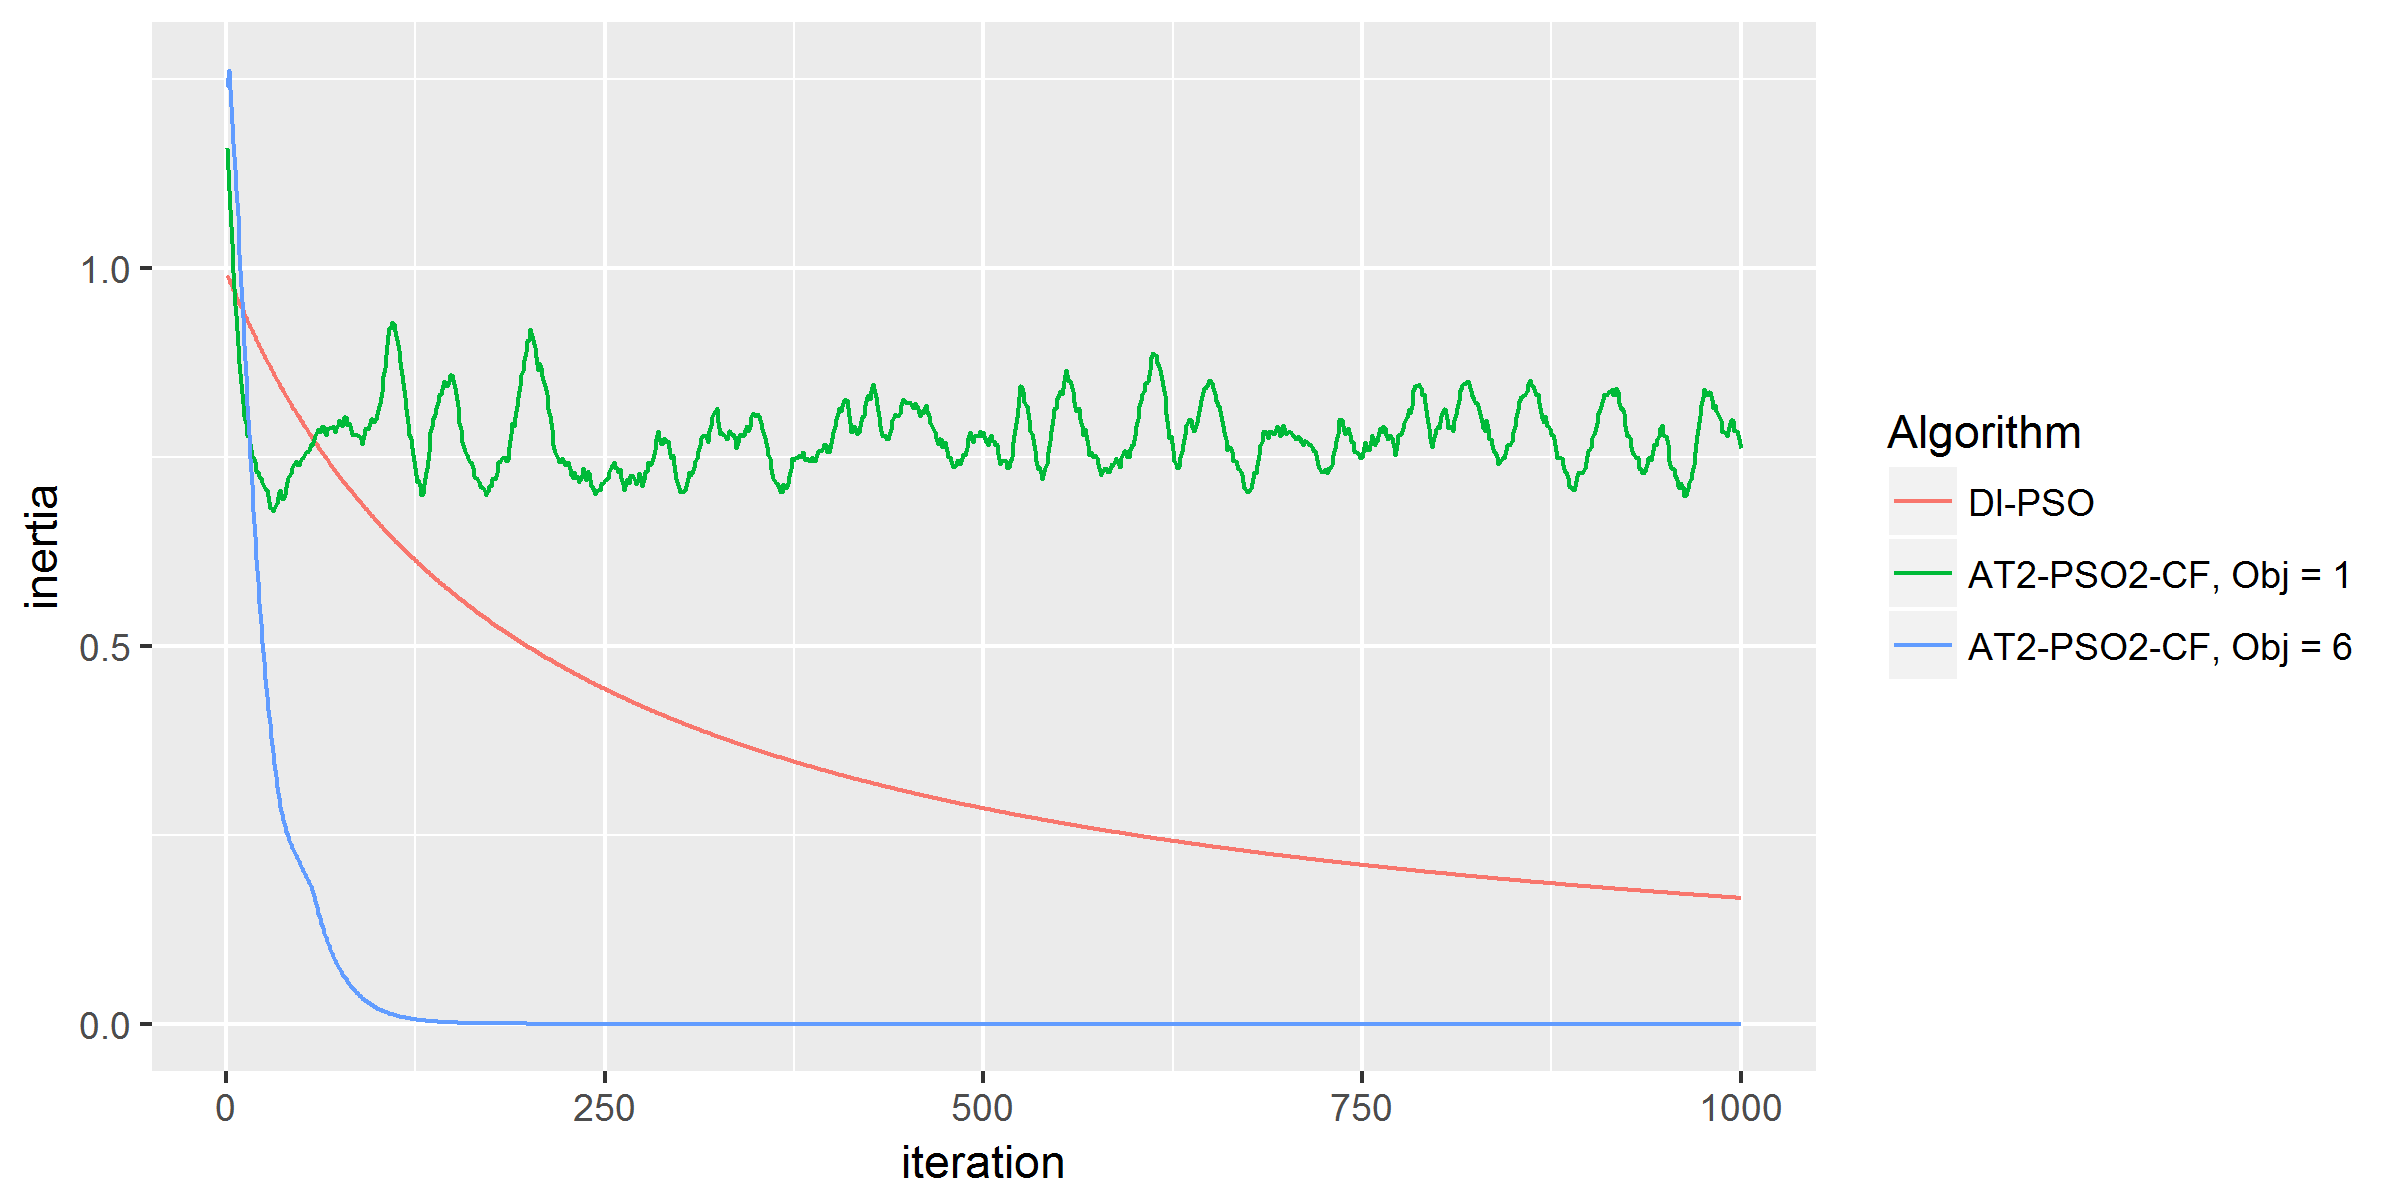
\includegraphics[width=0.95\textwidth]{code/psosims/inertiaplot.png}
\caption{Inertia over time for the DI-PSO algorithm with $\alpha=200$ and $\beta=1$, and for one replication of the AT-PSO-0.5 algorithm for each of OFs 1 and 6.}
\label{fig:inertia}
\end{figure}


Based on these simulations, our default recommendation is to use AT-BBPSO-MC or AT-BBPSOxp-MC with $R^*=0.3$ or $0.5$ and $df=3$ or $df=5$ along with the global neighborhood. These algorithms will not always be the best of the PSO algorithms, but they will often be very good. AT-PSO with $R^*=0.3$ or $R^*=0.5$ with a restrictive neighborhood topology such as ring-3 also tends to be a very good choice, though perhaps less consistent than the AT-BBPSO variants. Default PSO also performs rather well and is a good baseline algorithm to use for comparisons.


\begin{table}[ht]
\centering
\tiny{
\begin{tabular}{r|rrrr|rrrr|rrrr}
\multicolumn{1}{l}{OF1} & \multicolumn{4}{c}{Global nbhd} & \multicolumn{4}{c}{Ring-3 nbhd} & \multicolumn{4}{c}{Ring-1 nbhd}\\
\hline
Algorithm & Mean & SD & $\widehat{p}$ & $\widehat{t}$ & Mean & SD & $\widehat{p}$ & $\widehat{t}$ & Mean & SD & $\widehat{p}$ & $\widehat{t}$ \\
  \hline
\multicolumn{1}{l|}{PSO} & 4015.81 & 3124.33 & 0.00 & $\infty$ & 0.00 & 0.01 & 0.98 & 362.00 & 0.01 & 0.01 & 0.78 & 488.50 \\ 
  \multicolumn{1}{l|}{BBPSO-MC} & 84517.26 & 8944.33 & 0.00 & $\infty$ & 83674.80 & 9956.73 & 0.00 & $\infty$ & 84784.51 & 9451.47 & 0.00 & $\infty$ \\ 
  \multicolumn{1}{l|}{BBPSOxp-MC} & 84104.44 & 8192.44 & 0.00 & $\infty$ & 82952.29 & 9655.82 & 0.00 & $\infty$ & 85886.72 & 7182.36 & 0.00 & $\infty$ \\ 
\hline
\multicolumn{1}{l|}{AT-BBPSO-MC} &&&&&&&&&&&&\\
  $df = 1,\enspace$ $R^* =0.1$ & 1.59 & 0.47 & 0.00 & $\infty$ & 2.08 & 0.73 & 0.00 & $\infty$ & 2.10 & 0.89 & 0.00 & $\infty$ \\ 
  $df = 1,\enspace$ $R^* =0.3$ & 0.00 & 0.00 & 1.00 & 445.00 & 0.01 & 0.00 & 0.96 & 467.00 & 0.01 & 0.01 & 0.54 & 499.50 \\ 
  $df = 1,\enspace$ $R^* =0.5$ & 0.00 & 0.00 & 1.00 & 289.00 & 0.00 & 0.00 & 1.00 & 309.50 & 0.00 & 0.00 & 1.00 & 348.00 \\ 
  $df = 1,\enspace$ $R^* =0.7$ & 0.00 & 0.00 & 1.00 & 223.00 & 0.00 & 0.00 & 1.00 & 256.00 & 0.00 & 0.00 & 1.00 & 329.00 \\ 
  $df = 3,\enspace$ $R^* =0.1$ & 6.92 & 2.41 & 0.00 & $\infty$ & 6.92 & 1.79 & 0.00 & $\infty$ & 5.10 & 2.02 & 0.00 & $\infty$ \\ 
  $df = 3,\enspace$ $R^* =0.3$ & 0.01 & 0.00 & 0.22 & $\infty$ & 0.02 & 0.01 & 0.06 & $\infty$ & 0.03 & 0.01 & 0.00 & $\infty$ \\ 
  $df = 3,\enspace$ $R^* =0.5$ & 0.00 & 0.00 & 1.00 & 331.50 & 0.00 & 0.00 & 1.00 & 347.50 & 0.00 & 0.00 & 1.00 & 387.50 \\ 
  $df = 3,\enspace$ $R^* =0.7$ & 0.00 & 0.00 & 1.00 & 259.50 & 0.00 & 0.00 & 1.00 & 288.50 & 0.00 & 0.00 & 1.00 & 400.50 \\ 
  $df = 5,\enspace$ $R^* =0.1$ & 11.50 & 2.93 & 0.00 & $\infty$ & 11.72 & 2.53 & 0.00 & $\infty$ & 8.14 & 2.55 & 0.00 & $\infty$ \\ 
  $df = 5,\enspace$ $R^* =0.3$ & 0.03 & 0.01 & 0.00 & $\infty$ & 0.04 & 0.01 & 0.00 & $\infty$ & 0.06 & 0.02 & 0.00 & $\infty$ \\ 
  $df = 5,\enspace$ $R^* =0.5$ & 0.00 & 0.00 & 1.00 & 356.50 & 0.00 & 0.00 & 1.00 & 368.50 & 0.00 & 0.00 & 1.00 & 415.50 \\ 
  $df = 5,\enspace$ $R^* =0.7$ & 0.00 & 0.00 & 1.00 & 288.50 & 0.00 & 0.00 & 1.00 & 326.50 & 222.69 & 288.53 & 0.02 & $\infty$ \\ 
  $df = \infty,$ $R^* =0.1$ & 42.86 & 10.31 & 0.00 & $\infty$ & 38.44 & 8.12 & 0.00 & $\infty$ & 20.28 & 8.59 & 0.00 & $\infty$ \\ 
  $df = \infty,$ $R^* =0.3$ & 0.14 & 0.05 & 0.00 & $\infty$ & 0.15 & 0.03 & 0.00 & $\infty$ & 0.25 & 0.08 & 0.00 & $\infty$ \\ 
  $df = \infty,$ $R^* =0.5$ & 0.00 & 0.00 & 1.00 & 415.00 & 0.00 & 0.00 & 1.00 & 433.00 & 0.01 & 0.00 & 0.94 & 489.00 \\ 
  $df = \infty,$ $R^* =0.7$ & 0.00 & 0.00 & 1.00 & 352.00 & 0.00 & 0.00 & 0.98 & 441.50 & 16949.57 & 3141.36 & 0.00 & $\infty$ \\ 
\hline
\multicolumn{1}{l|}{AT-BBPSOxp-MC} &&&&&&&&&&&&\\
  $df = 1,\enspace$ $R^* =0.1$ & 5.71 & 1.58 & 0.00 & $\infty$ & 6.00 & 1.76 & 0.00 & $\infty$ & 3.91 & 1.75 & 0.00 & $\infty$ \\ 
  $df = 1,\enspace$ $R^* =0.3$ & 0.02 & 0.01 & 0.00 & $\infty$ & 0.04 & 0.01 & 0.00 & $\infty$ & 0.05 & 0.02 & 0.00 & $\infty$ \\ 
  $df = 1,\enspace$ $R^* =0.5$ & 0.00 & 0.00 & 1.00 & 358.00 & 0.00 & 0.00 & 1.00 & 381.00 & 0.00 & 0.00 & 1.00 & 419.50 \\ 
  $df = 1,\enspace$ $R^* =0.7$ & 0.00 & 0.00 & 1.00 & 291.00 & 0.00 & 0.00 & 1.00 & 326.00 & 0.00 & 0.01 & 0.98 & 432.50 \\ 
  $df = 3,\enspace$ $R^* =0.1$ & 17.42 & 4.87 & 0.00 & $\infty$ & 16.91 & 4.41 & 0.00 & $\infty$ & 8.64 & 3.12 & 0.00 & $\infty$ \\ 
  $df = 3,\enspace$ $R^* =0.3$ & 0.10 & 0.03 & 0.00 & $\infty$ & 0.12 & 0.04 & 0.00 & $\infty$ & 0.15 & 0.05 & 0.00 & $\infty$ \\ 
  $df = 3,\enspace$ $R^* =0.5$ & 0.00 & 0.00 & 1.00 & 412.00 & 0.00 & 0.00 & 1.00 & 431.50 & 0.01 & 0.00 & 0.92 & 470.50 \\ 
  $df = 3,\enspace$ $R^* =0.7$ & 0.00 & 0.00 & 1.00 & 350.50 & 0.00 & 0.01 & 0.98 & 438.00 & 4193.16 & 2013.59 & 0.00 & $\infty$ \\ 
  $df = 5,\enspace$ $R^* =0.1$ & 28.39 & 6.37 & 0.00 & $\infty$ & 28.42 & 7.58 & 0.00 & $\infty$ & 13.22 & 5.27 & 0.00 & $\infty$ \\ 
  $df = 5,\enspace$ $R^* =0.3$ & 0.19 & 0.05 & 0.00 & $\infty$ & 0.22 & 0.07 & 0.00 & $\infty$ & 0.26 & 0.10 & 0.00 & $\infty$ \\ 
  $df = 5,\enspace$ $R^* =0.5$ & 0.00 & 0.00 & 1.00 & 440.00 & 0.00 & 0.00 & 1.00 & 466.00 & 0.03 & 0.02 & 0.04 & $\infty$ \\ 
  $df = 5,\enspace$ $R^* =0.7$ & 0.00 & 0.00 & 1.00 & 405.50 & 505.43 & 755.11 & 0.02 & $\infty$ & 17674.52 & 4505.53 & 0.00 & $\infty$ \\ 
  $df = \infty,$ $R^* =0.1$ & 65.18 & 14.92 & 0.00 & $\infty$ & 60.90 & 13.82 & 0.00 & $\infty$ & 26.77 & 10.11 & 0.00 & $\infty$ \\ 
  $df = \infty,$ $R^* =0.3$ & 0.50 & 0.11 & 0.00 & $\infty$ & 0.66 & 0.14 & 0.00 & $\infty$ & 0.82 & 0.25 & 0.00 & $\infty$ \\ 
  $df = \infty,$ $R^* =0.5$ & 0.01 & 0.00 & 0.82 & 492.00 & 0.03 & 0.01 & 0.02 & $\infty$ & 0.85 & 0.75 & 0.00 & $\infty$ \\ 
  $df = \infty,$ $R^* =0.7$ & 0.19 & 0.33 & 0.04 & $\infty$ & 17369.34 & 3631.71 & 0.00 & $\infty$ & 35172.80 & 4377.92 & 0.00 & $\infty$ \\ 
\hline
\multicolumn{1}{l|}{DI-PSO} &&&&&&&&&&&&\\
  $\alpha = 50,\enspace$ $\beta =1$ & 6703.90 & 3993.99 & 0.00 & $\infty$ & 543.02 & 683.48 & 0.00 & $\infty$ & 51.63 & 95.71 & 0.00 & $\infty$ \\ 
  $\alpha = 50,\enspace$ $\beta =2$ & 7823.89 & 4787.27 & 0.00 & $\infty$ & 1821.42 & 1508.50 & 0.00 & $\infty$ & 499.64 & 441.33 & 0.00 & $\infty$ \\ 
  $\alpha = 50,\enspace$ $\beta =4$ & 15373.54 & 6906.92 & 0.00 & $\infty$ & 5572.40 & 3137.25 & 0.00 & $\infty$ & 3705.93 & 2324.41 & 0.00 & $\infty$ \\ 
  $\alpha = 100,$ $\beta =1$ & 3928.51 & 3855.22 & 0.00 & $\infty$ & 236.79 & 733.83 & 0.00 & $\infty$ & 0.99 & 4.03 & 0.20 & $\infty$ \\ 
  $\alpha = 100,$ $\beta =2$ & 7618.89 & 4250.92 & 0.00 & $\infty$ & 1206.09 & 1393.42 & 0.00 & $\infty$ & 84.99 & 137.32 & 0.00 & $\infty$ \\ 
  $\alpha = 100,$ $\beta =4$ & 13044.34 & 6195.43 & 0.00 & $\infty$ & 4218.13 & 2881.34 & 0.00 & $\infty$ & 1745.64 & 1532.00 & 0.00 & $\infty$ \\ 
  $\alpha = 200,$ $\beta =1$ & 2321.68 & 2088.02 & 0.00 & $\infty$ & 178.09 & 618.06 & 0.02 & $\infty$ & 0.00 & 0.00 & 1.00 & 383.50 \\ 
  $\alpha = 200,$ $\beta =2$ & 6427.62 & 3741.12 & 0.00 & $\infty$ & 305.62 & 523.71 & 0.00 & $\infty$ & 5.45 & 12.55 & 0.00 & $\infty$ \\ 
  $\alpha = 200,$ $\beta =4$ & 12004.75 & 5708.12 & 0.00 & $\infty$ & 2236.94 & 1729.58 & 0.00 & $\infty$ & 475.93 & 503.87 & 0.00 & $\infty$ \\ 
\hline
\multicolumn{1}{l|}{AT-PSO} &&&&&&&&&&&&\\
  $R^* = 0.1$ & 111.02 & 237.73 & 0.00 & $\infty$ & 211.79 & 889.18 & 0.00 & $\infty$ & 12223.23 & 9590.30 & 0.00 & $\infty$ \\ 
  $R^* = 0.3$ & 54.27 & 252.08 & 0.04 & $\infty$ & 0.00 & 0.00 & 1.00 & 347.00 & 0.00 & 0.01 & 0.88 & 457.00 \\ 
  $R^* = 0.5$ & 329.77 & 586.04 & 0.00 & $\infty$ & 0.00 & 0.00 & 1.00 & 274.50 & 0.00 & 0.00 & 1.00 & 303.50 \\ 
  $R^* = 0.7$ & 2131.94 & 2209.74 & 0.00 & $\infty$ & 0.04 & 0.21 & 0.92 & 381.50 & 0.00 & 0.00 & 1.00 & 341.50 \\ 
   \hline
\end{tabular}
}
\caption{Simulation results for OF1. See text for description.}
\label{tab:psosim1}
\end{table}
% latex table generated in R 3.3.1 by xtable 1.8-2 package
% Sun Aug 21 22:17:27 2016
\begin{table}[ht]
\centering
\tiny{
\begin{tabular}{r|rrrr|rrrr|rrrr}
\multicolumn{1}{l}{OF2} & \multicolumn{4}{c}{Global nbhd} & \multicolumn{4}{c}{Ring-3 nbhd} & \multicolumn{4}{c}{Ring-1 nbhd}\\
  \hline
Algorithm & Mean & SD & $\widehat{p}$ & $\widehat{t}$ & Mean & SD & $\widehat{p}$ & $\widehat{t}$ & Mean & SD & $\widehat{p}$ & $\widehat{t}$ \\
  \hline
\multicolumn{1}{l|}{PSO} & 10915.05 & 17201.47 & 0.00 & $\infty$ & 1246.38 & 1002.75 & 0.00 & $\infty$ & 5738.34 & 3835.37 & 0.00 & $\infty$ \\ 
  \multicolumn{1}{l|}{BBPSO-MC} & 9081909.83 & 1958288.73 & 0.00 & $\infty$ & 9194595.70 & 2157840.19 & 0.00 & $\infty$ & 8830368.63 & 2234188.42 & 0.00 & $\infty$ \\ 
  \multicolumn{1}{l|}{BBPSOxp-MC} & 9138885.89 & 2265920.11 & 0.00 & $\infty$ & 8889637.56 & 2035964.50 & 0.00 & $\infty$ & 9038770.99 & 1858659.66 & 0.00 & $\infty$ \\ 
\hline
\multicolumn{1}{l|}{AT-BBPSO-MC} &&&&&&&&&&&&\\
  $df = 1,\enspace$ $R^* =0.1$ & 950.30 & 809.12 & 0.00 & $\infty$ & 690.95 & 535.97 & 0.00 & $\infty$ & 743.12 & 728.28 & 0.00 & $\infty$ \\ 
  $df = 1,\enspace$ $R^* =0.3$ & 300.03 & 258.36 & 0.00 & $\infty$ & 685.68 & 458.39 & 0.00 & $\infty$ & 1091.45 & 1375.54 & 0.00 & $\infty$ \\ 
  $df = 1,\enspace$ $R^* =0.5$ & 440.38 & 436.08 & 0.00 & $\infty$ & 1419.88 & 1239.43 & 0.00 & $\infty$ & 3652.45 & 4072.28 & 0.00 & $\infty$ \\ 
  $df = 1,\enspace$ $R^* =0.7$ & 1615.81 & 1539.22 & 0.00 & $\infty$ & 4330.31 & 4863.92 & 0.00 & $\infty$ & 8858.46 & 4578.27 & 0.00 & $\infty$ \\ 
  $df = 3,\enspace$ $R^* =0.1$ & 196.07 & 88.33 & 0.00 & $\infty$ & 226.17 & 163.16 & 0.00 & $\infty$ & 252.63 & 187.08 & 0.00 & $\infty$ \\ 
  $df = 3,\enspace$ $R^* =0.3$ & 23.27 & 17.11 & 0.00 & $\infty$ & 54.95 & 48.43 & 0.00 & $\infty$ & 189.83 & 399.03 & 0.00 & $\infty$ \\ 
  $df = 3,\enspace$ $R^* =0.5$ & 30.94 & 29.21 & 0.00 & $\infty$ & 185.87 & 161.77 & 0.00 & $\infty$ & 1073.22 & 1233.74 & 0.00 & $\infty$ \\ 
  $df = 3,\enspace$ $R^* =0.7$ & 222.12 & 524.53 & 0.00 & $\infty$ & 939.33 & 789.54 & 0.00 & $\infty$ & 5897.58 & 4513.86 & 0.00 & $\infty$ \\ 
  $df = 5,\enspace$ $R^* =0.1$ & 198.27 & 75.35 & 0.00 & $\infty$ & 175.31 & 80.21 & 0.00 & $\infty$ & 205.86 & 117.06 & 0.00 & $\infty$ \\ 
  $df = 5,\enspace$ $R^* =0.3$ & 12.25 & 9.35 & 0.00 & $\infty$ & 24.76 & 18.02 & 0.00 & $\infty$ & 60.79 & 63.04 & 0.00 & $\infty$ \\ 
  $df = 5,\enspace$ $R^* =0.5$ & 11.51 & 7.41 & 0.00 & $\infty$ & 63.91 & 51.53 & 0.00 & $\infty$ & 458.47 & 317.21 & 0.00 & $\infty$ \\ 
  $df = 5,\enspace$ $R^* =0.7$ & 61.67 & 36.27 & 0.00 & $\infty$ & 378.27 & 218.82 & 0.00 & $\infty$ & 7696.71 & 5485.99 & 0.00 & $\infty$ \\ 
  $df = \infty,$ $R^* =0.1$ & 280.79 & 97.77 & 0.00 & $\infty$ & 267.44 & 87.93 & 0.00 & $\infty$ & 287.37 & 128.28 & 0.00 & $\infty$ \\ 
  $df = \infty,$ $R^* =0.3$ & 6.75 & 3.83 & 0.00 & $\infty$ & 13.91 & 9.02 & 0.00 & $\infty$ & 39.37 & 32.01 & 0.00 & $\infty$ \\ 
  $df = \infty,$ $R^* =0.5$ & 4.96 & 3.73 & 0.00 & $\infty$ & 30.82 & 22.83 & 0.00 & $\infty$ & 269.58 & 161.10 & 0.00 & $\infty$ \\ 
  $df = \infty,$ $R^* =0.7$ & 51.31 & 38.92 & 0.00 & $\infty$ & 550.48 & 301.85 & 0.00 & $\infty$ & 1100097.72 & 493290.33 & 0.00 & $\infty$ \\ 
\hline
\multicolumn{1}{l|}{AT-BBPSOxp-MC} &&&&&&&&&&&&\\
  $df = 1,\enspace$ $R^* =0.1$ & 1620.04 & 724.59 & 0.00 & $\infty$ & 1434.81 & 637.94 & 0.00 & $\infty$ & 1004.77 & 608.51 & 0.00 & $\infty$ \\ 
  $df = 1,\enspace$ $R^* =0.3$ & 1117.65 & 614.18 & 0.00 & $\infty$ & 1541.55 & 913.10 & 0.00 & $\infty$ & 1372.47 & 1108.92 & 0.00 & $\infty$ \\ 
  $df = 1,\enspace$ $R^* =0.5$ & 2424.76 & 1458.65 & 0.00 & $\infty$ & 3639.53 & 2048.74 & 0.00 & $\infty$ & 5212.21 & 3221.11 & 0.00 & $\infty$ \\ 
  $df = 1,\enspace$ $R^* =0.7$ & 5685.79 & 3365.32 & 0.00 & $\infty$ & 6746.82 & 4254.76 & 0.00 & $\infty$ & 13170.58 & 7291.81 & 0.00 & $\infty$ \\ 
  $df = 3,\enspace$ $R^* =0.1$ & 609.04 & 289.92 & 0.00 & $\infty$ & 568.65 & 326.15 & 0.00 & $\infty$ & 562.17 & 301.77 & 0.00 & $\infty$ \\ 
  $df = 3,\enspace$ $R^* =0.3$ & 231.40 & 167.47 & 0.00 & $\infty$ & 320.46 & 308.01 & 0.00 & $\infty$ & 366.68 & 274.58 & 0.00 & $\infty$ \\ 
  $df = 3,\enspace$ $R^* =0.5$ & 360.34 & 224.38 & 0.00 & $\infty$ & 1026.42 & 709.48 & 0.00 & $\infty$ & 5089.66 & 5857.62 & 0.00 & $\infty$ \\ 
  $df = 3,\enspace$ $R^* =0.7$ & 1426.88 & 1209.92 & 0.00 & $\infty$ & 5568.83 & 7882.29 & 0.00 & $\infty$ & 38081.89 & 31747.85 & 0.00 & $\infty$ \\ 
  $df = 5,\enspace$ $R^* =0.1$ & 476.81 & 215.75 & 0.00 & $\infty$ & 497.74 & 194.10 & 0.00 & $\infty$ & 540.99 & 263.49 & 0.00 & $\infty$ \\ 
  $df = 5,\enspace$ $R^* =0.3$ & 109.01 & 45.98 & 0.00 & $\infty$ & 170.67 & 120.10 & 0.00 & $\infty$ & 272.26 & 192.17 & 0.00 & $\infty$ \\ 
  $df = 5,\enspace$ $R^* =0.5$ & 243.73 & 154.52 & 0.00 & $\infty$ & 448.77 & 241.51 & 0.00 & $\infty$ & 2147.17 & 1308.53 & 0.00 & $\infty$ \\ 
  $df = 5,\enspace$ $R^* =0.7$ & 794.68 & 388.65 & 0.00 & $\infty$ & 17971.50 & 16875.10 & 0.00 & $\infty$ & 507347.01 & 409181.08 & 0.00 & $\infty$ \\ 
  $df = \infty,$ $R^* =0.1$ & 609.19 & 197.59 & 0.00 & $\infty$ & 585.88 & 163.05 & 0.00 & $\infty$ & 536.88 & 263.19 & 0.00 & $\infty$ \\ 
  $df = \infty,$ $R^* =0.3$ & 70.82 & 44.69 & 0.00 & $\infty$ & 111.39 & 79.50 & 0.00 & $\infty$ & 220.30 & 168.06 & 0.00 & $\infty$ \\ 
  $df = \infty,$ $R^* =0.5$ & 114.86 & 88.86 & 0.00 & $\infty$ & 329.69 & 169.04 & 0.00 & $\infty$ & 2889.16 & 2088.86 & 0.00 & $\infty$ \\ 
  $df = \infty,$ $R^* =0.7$ & 2469.49 & 2799.80 & 0.00 & $\infty$ & 1483405.94 & 407996.51 & 0.00 & $\infty$ & 2535125.64 & 778910.46 & 0.00 & $\infty$ \\ 
\hline
\multicolumn{1}{l|}{DI-PSO} &&&&&&&&&&&&\\
  $\alpha = 50,\enspace$ $\beta =1$ & 40714.56 & 24208.86 & 0.00 & $\infty$ & 16548.67 & 9312.34 & 0.00 & $\infty$ & 7839.43 & 5031.49 & 0.00 & $\infty$ \\ 
  $\alpha = 50,\enspace$ $\beta =2$ & 47763.21 & 31361.92 & 0.00 & $\infty$ & 24627.59 & 11610.10 & 0.00 & $\infty$ & 11660.25 & 6362.56 & 0.00 & $\infty$ \\ 
  $\alpha = 50,\enspace$ $\beta =4$ & 62225.74 & 28459.35 & 0.00 & $\infty$ & 31511.13 & 15145.07 & 0.00 & $\infty$ & 16416.52 & 7831.71 & 0.00 & $\infty$ \\ 
  $\alpha = 100,$ $\beta =1$ & 26613.11 & 14611.63 & 0.00 & $\infty$ & 10168.37 & 6029.10 & 0.00 & $\infty$ & 5378.87 & 3302.21 & 0.00 & $\infty$ \\ 
  $\alpha = 100,$ $\beta =2$ & 46177.71 & 37974.29 & 0.00 & $\infty$ & 17795.63 & 8897.56 & 0.00 & $\infty$ & 9818.51 & 4708.72 & 0.00 & $\infty$ \\ 
  $\alpha = 100,$ $\beta =4$ & 64833.73 & 36534.52 & 0.00 & $\infty$ & 28627.71 & 14257.04 & 0.00 & $\infty$ & 14536.17 & 7921.94 & 0.00 & $\infty$ \\ 
  $\alpha = 200,$ $\beta =1$ & 21611.55 & 12914.90 & 0.00 & $\infty$ & 5699.97 & 3916.44 & 0.00 & $\infty$ & 3499.49 & 1865.32 & 0.00 & $\infty$ \\ 
  $\alpha = 200,$ $\beta =2$ & 36405.44 & 27997.69 & 0.00 & $\infty$ & 12492.90 & 6829.93 & 0.00 & $\infty$ & 6944.87 & 4559.84 & 0.00 & $\infty$ \\ 
  $\alpha = 200,$ $\beta =4$ & 57723.16 & 30860.32 & 0.00 & $\infty$ & 21807.81 & 11567.18 & 0.00 & $\infty$ & 12201.41 & 5365.69 & 0.00 & $\infty$ \\ 
\hline
\multicolumn{1}{l|}{AT-PSO} &&&&&&&&&&&&\\
  $R^* = 0.1$ & 8823.66 & 9727.43 & 0.00 & $\infty$ & 8852.96 & 6912.25 & 0.00 & $\infty$ & 58369.56 & 38288.17 & 0.00 & $\infty$ \\ 
  $R^* = 0.3$ & 6658.84 & 6659.87 & 0.00 & $\infty$ & 769.74 & 850.01 & 0.00 & $\infty$ & 5183.03 & 4046.47 & 0.00 & $\infty$ \\ 
  $R^* = 0.5$ & 20994.61 & 16398.66 & 0.00 & $\infty$ & 1713.89 & 2589.20 & 0.00 & $\infty$ & 1877.08 & 1465.51 & 0.00 & $\infty$ \\ 
  $R^* = 0.7$ & 35128.87 & 17886.90 & 0.00 & $\infty$ & 7126.76 & 5756.50 & 0.00 & $\infty$ & 5771.37 & 3581.95 & 0.00 & $\infty$ \\ 
   \hline
\end{tabular}
}
\caption{Simulation results for OF2. See text for description.}
\label{tab:psosim2}
\end{table}
% latex table generated in R 3.3.1 by xtable 1.8-2 package
% Sun Aug 21 22:17:27 2016
\begin{table}[ht]
\centering
\tiny{
\begin{tabular}{r|rrrr|rrrr|rrrr}
\multicolumn{1}{l}{OF3} & \multicolumn{4}{c}{Global nbhd} & \multicolumn{4}{c}{Ring-3 nbhd} & \multicolumn{4}{c}{Ring-1 nbhd}\\
  \hline
Algorithm & Mean & SD & $\widehat{p}$ & $\widehat{t}$ & Mean & SD & $\widehat{p}$ & $\widehat{t}$ & Mean & SD & $\widehat{p}$ & $\widehat{t}$ \\ 
  \hline
\multicolumn{1}{l|}{PSO} & 1242764.67 & 2075592.00 & 0.00 & $\infty$ & 121.33 & 104.18 & 0.00 & $\infty$ & 241.45 & 255.69 & 0.00 & $\infty$ \\ 
  \multicolumn{1}{l|}{BBPSO-MC} & 232830400.95 & 37473167.09 & 0.00 & $\infty$ & 247662755.14 & 43820300.43 & 0.00 & $\infty$ & 247321508.63 & 39096259.33 & 0.00 & $\infty$ \\ 
  \multicolumn{1}{l|}{BBPSOxp-MC} & 235491326.54 & 42124202.61 & 0.00 & $\infty$ & 242679907.63 & 42872974.55 & 0.00 & $\infty$ & 253599464.23 & 43615037.04 & 0.00 & $\infty$ \\ 
\hline
\multicolumn{1}{l|}{AT-BBPSO-MC} &&&&&&&&&&&&\\
  $df = 1,\enspace$ $R^* =0.1$ & 382.54 & 325.35 & 0.00 & $\infty$ & 486.70 & 533.46 & 0.00 & $\infty$ & 669.09 & 932.66 & 0.00 & $\infty$ \\ 
  $df = 1,\enspace$ $R^* =0.3$ & 233.17 & 429.80 & 0.00 & $\infty$ & 182.89 & 272.06 & 0.00 & $\infty$ & 352.64 & 465.63 & 0.00 & $\infty$ \\ 
  $df = 1,\enspace$ $R^* =0.5$ & 315.43 & 497.55 & 0.00 & $\infty$ & 159.55 & 216.03 & 0.00 & $\infty$ & 254.78 & 669.72 & 0.00 & $\infty$ \\ 
  $df = 1,\enspace$ $R^* =0.7$ & 235.08 & 455.38 & 0.00 & $\infty$ & 96.32 & 106.25 & 0.00 & $\infty$ & 189.20 & 288.45 & 0.00 & $\infty$ \\ 
  $df = 3,\enspace$ $R^* =0.1$ & 545.05 & 481.33 & 0.00 & $\infty$ & 629.79 & 657.37 & 0.00 & $\infty$ & 567.75 & 585.07 & 0.00 & $\infty$ \\ 
  $df = 3,\enspace$ $R^* =0.3$ & 176.81 & 186.22 & 0.00 & $\infty$ & 172.84 & 204.18 & 0.00 & $\infty$ & 256.32 & 426.46 & 0.00 & $\infty$ \\ 
  $df = 3,\enspace$ $R^* =0.5$ & 159.09 & 170.77 & 0.00 & $\infty$ & 128.99 & 127.25 & 0.00 & $\infty$ & 137.56 & 202.68 & 0.00 & $\infty$ \\ 
  $df = 3,\enspace$ $R^* =0.7$ & 155.74 & 399.33 & 0.00 & $\infty$ & 132.16 & 339.64 & 0.00 & $\infty$ & 82.12 & 170.21 & 0.00 & $\infty$ \\ 
  $df = 5,\enspace$ $R^* =0.1$ & 833.71 & 627.25 & 0.00 & $\infty$ & 928.42 & 982.63 & 0.00 & $\infty$ & 450.93 & 444.86 & 0.00 & $\infty$ \\ 
  $df = 5,\enspace$ $R^* =0.3$ & 283.78 & 431.37 & 0.00 & $\infty$ & 135.95 & 98.01 & 0.00 & $\infty$ & 229.39 & 314.25 & 0.00 & $\infty$ \\ 
  $df = 5,\enspace$ $R^* =0.5$ & 198.53 & 185.97 & 0.00 & $\infty$ & 173.66 & 278.73 & 0.00 & $\infty$ & 118.79 & 114.49 & 0.00 & $\infty$ \\ 
  $df = 5,\enspace$ $R^* =0.7$ & 142.06 & 190.31 & 0.00 & $\infty$ & 64.57 & 98.26 & 0.00 & $\infty$ & 108.71 & 538.33 & 0.00 & $\infty$ \\ 
  $df = \infty,$ $R^* =0.1$ & 1343.31 & 757.87 & 0.00 & $\infty$ & 1056.96 & 522.89 & 0.00 & $\infty$ & 958.18 & 773.33 & 0.00 & $\infty$ \\ 
  $df = \infty,$ $R^* =0.3$ & 230.32 & 320.08 & 0.00 & $\infty$ & 138.02 & 120.68 & 0.00 & $\infty$ & 212.78 & 331.90 & 0.00 & $\infty$ \\ 
  $df = \infty,$ $R^* =0.5$ & 225.28 & 219.75 & 0.00 & $\infty$ & 156.78 & 132.24 & 0.00 & $\infty$ & 120.23 & 106.23 & 0.00 & $\infty$ \\ 
  $df = \infty,$ $R^* =0.7$ & 131.34 & 91.53 & 0.00 & $\infty$ & 56.10 & 76.80 & 0.00 & $\infty$ & 179.69 & 683.04 & 0.00 & $\infty$ \\ 
\hline
\multicolumn{1}{l|}{AT-BBPSOxp-MC} &&&&&&&&&&&&\\
  $df = 1,\enspace$ $R^* =0.1$ & 616.80 & 278.83 & 0.00 & $\infty$ & 633.00 & 276.25 & 0.00 & $\infty$ & 490.75 & 350.79 & 0.00 & $\infty$ \\ 
  $df = 1,\enspace$ $R^* =0.3$ & 152.80 & 179.75 & 0.00 & $\infty$ & 163.64 & 131.42 & 0.00 & $\infty$ & 140.13 & 158.06 & 0.00 & $\infty$ \\ 
  $df = 1,\enspace$ $R^* =0.5$ & 139.49 & 269.65 & 0.00 & $\infty$ & 99.39 & 225.41 & 0.00 & $\infty$ & 202.26 & 429.55 & 0.00 & $\infty$ \\ 
  $df = 1,\enspace$ $R^* =0.7$ & 149.01 & 459.29 & 0.00 & $\infty$ & 73.54 & 126.07 & 0.00 & $\infty$ & 188.28 & 370.67 & 0.00 & $\infty$ \\ 
  $df = 3,\enspace$ $R^* =0.1$ & 961.94 & 370.97 & 0.00 & $\infty$ & 931.38 & 294.49 & 0.00 & $\infty$ & 709.41 & 452.45 & 0.00 & $\infty$ \\ 
  $df = 3,\enspace$ $R^* =0.3$ & 168.44 & 279.24 & 0.00 & $\infty$ & 144.15 & 200.78 & 0.00 & $\infty$ & 120.33 & 48.68 & 0.00 & $\infty$ \\ 
  $df = 3,\enspace$ $R^* =0.5$ & 123.39 & 102.98 & 0.00 & $\infty$ & 97.56 & 50.88 & 0.00 & $\infty$ & 77.47 & 81.83 & 0.00 & $\infty$ \\ 
  $df = 3,\enspace$ $R^* =0.7$ & 49.75 & 70.72 & 0.00 & $\infty$ & 33.96 & 52.12 & 0.00 & $\infty$ & 3586.02 & 9973.24 & 0.00 & $\infty$ \\ 
  $df = 5,\enspace$ $R^* =0.1$ & 1229.87 & 526.97 & 0.00 & $\infty$ & 1171.93 & 406.81 & 0.00 & $\infty$ & 727.95 & 436.07 & 0.00 & $\infty$ \\ 
  $df = 5,\enspace$ $R^* =0.3$ & 267.86 & 435.67 & 0.00 & $\infty$ & 124.80 & 75.86 & 0.00 & $\infty$ & 157.72 & 217.77 & 0.00 & $\infty$ \\ 
  $df = 5,\enspace$ $R^* =0.5$ & 137.08 & 104.13 & 0.00 & $\infty$ & 91.44 & 86.38 & 0.00 & $\infty$ & 75.74 & 95.04 & 0.00 & $\infty$ \\ 
  $df = 5,\enspace$ $R^* =0.7$ & 66.87 & 126.23 & 0.00 & $\infty$ & 19.28 & 17.08 & 0.00 & $\infty$ & 82498.29 & 102684.12 & 0.00 & $\infty$ \\ 
  $df = \infty,$ $R^* =0.1$ & 2002.70 & 822.46 & 0.00 & $\infty$ & 1718.67 & 698.34 & 0.00 & $\infty$ & 1158.47 & 903.16 & 0.00 & $\infty$ \\ 
  $df = \infty,$ $R^* =0.3$ & 137.09 & 84.51 & 0.00 & $\infty$ & 116.46 & 66.60 & 0.00 & $\infty$ & 114.47 & 57.68 & 0.00 & $\infty$ \\ 
  $df = \infty,$ $R^* =0.5$ & 121.71 & 103.55 & 0.00 & $\infty$ & 104.78 & 67.31 & 0.00 & $\infty$ & 41.15 & 33.00 & 0.00 & $\infty$ \\ 
  $df = \infty,$ $R^* =0.7$ & 24.31 & 24.58 & 0.00 & $\infty$ & 24.31 & 20.57 & 0.00 & $\infty$ & 2088154.00 & 1258187.91 & 0.00 & $\infty$ \\ 
\hline
\multicolumn{1}{l|}{DI-PSO} &&&&&&&&&&&&\\
  $\alpha = 50,\enspace$ $\beta =1$ & 4180196.82 & 4677639.48 & 0.00 & $\infty$ & 354071.40 & 579847.34 & 0.00 & $\infty$ & 70128.62 & 165037.08 & 0.00 & $\infty$ \\ 
  $\alpha = 50,\enspace$ $\beta =2$ & 6964209.15 & 8322398.93 & 0.00 & $\infty$ & 2341768.78 & 4277548.98 & 0.00 & $\infty$ & 1232022.80 & 1464906.82 & 0.00 & $\infty$ \\ 
  $\alpha = 50,\enspace$ $\beta =4$ & 20143670.82 & 15026478.57 & 0.00 & $\infty$ & 11740754.91 & 8374232.25 & 0.00 & $\infty$ & 6766696.51 & 4472751.26 & 0.00 & $\infty$ \\ 
  $\alpha = 100,$ $\beta =1$ & 1610827.18 & 3342137.70 & 0.00 & $\infty$ & 55104.82 & 171942.01 & 0.00 & $\infty$ & 1691.16 & 3160.57 & 0.00 & $\infty$ \\ 
  $\alpha = 100,$ $\beta =2$ & 6945649.64 & 6844592.19 & 0.00 & $\infty$ & 1001725.17 & 1774982.73 & 0.00 & $\infty$ & 150478.59 & 213009.16 & 0.00 & $\infty$ \\ 
  $\alpha = 100,$ $\beta =4$ & 21536033.79 & 15337048.80 & 0.00 & $\infty$ & 6691579.83 & 5932202.88 & 0.00 & $\infty$ & 4328277.03 & 4060546.38 & 0.00 & $\infty$ \\ 
  $\alpha = 200,$ $\beta =1$ & 1543367.07 & 2077471.63 & 0.00 & $\infty$ & 4350.55 & 16257.10 & 0.00 & $\infty$ & 266.44 & 453.75 & 0.00 & $\infty$ \\ 
  $\alpha = 200,$ $\beta =2$ & 6626917.67 & 9093854.31 & 0.00 & $\infty$ & 299834.83 & 1040979.02 & 0.00 & $\infty$ & 5848.88 & 14329.18 & 0.00 & $\infty$ \\ 
  $\alpha = 200,$ $\beta =4$ & 17830796.63 & 14245007.26 & 0.00 & $\infty$ & 3367710.63 & 3194612.95 & 0.00 & $\infty$ & 776424.69 & 865443.75 & 0.00 & $\infty$ \\ 
\hline
\multicolumn{1}{l|}{AT-PSO} &&&&&&&&&&&&\\
  $R^* = 0.1$ & 5779.95 & 14928.86 & 0.00 & $\infty$ & 297272.41 & 1261108.56 & 0.00 & $\infty$ & 33785179.04 & 23020834.78 & 0.00 & $\infty$ \\ 
  $R^* = 0.3$ & 869.69 & 2100.98 & 0.00 & $\infty$ & 131.15 & 175.33 & 0.00 & $\infty$ & 184.15 & 186.17 & 0.00 & $\infty$ \\ 
  $R^* = 0.5$ & 71363.37 & 218211.42 & 0.00 & $\infty$ & 190.13 & 271.20 & 0.00 & $\infty$ & 134.32 & 200.92 & 0.00 & $\infty$ \\ 
  $R^* = 0.7$ & 1572669.78 & 3884482.27 & 0.00 & $\infty$ & 391.10 & 857.02 & 0.00 & $\infty$ & 535.09 & 1277.83 & 0.00 & $\infty$ \\ 
   \hline
\end{tabular}
}
\caption{Simulation results for OF3. See text for description.}
\label{tab:psosim3}
\end{table}
% latex table generated in R 3.3.1 by xtable 1.8-2 package
% Sun Aug 21 22:17:27 2016
\begin{table}[ht]
\centering
\tiny{
\begin{tabular}{r|rrrr|rrrr|rrrr}
\multicolumn{1}{l}{OF4} & \multicolumn{4}{c}{Global nbhd} & \multicolumn{4}{c}{Ring-3 nbhd} & \multicolumn{4}{c}{Ring-1 nbhd}\\
  \hline
Algorithm & Mean & SD & $\widehat{p}$ & $\widehat{t}$ & Mean & SD & $\widehat{p}$ & $\widehat{t}$ & Mean & SD & $\widehat{p}$ & $\widehat{t}$ \\ 
  \hline
\multicolumn{1}{l|}{PSO} & 29.94 & 15.21 & 0.00 & $\infty$ & 5.37 & 3.47 & 0.02 & $\infty$ & 3.24 & 1.44 & 0.00 & $\infty$ \\ 
  \multicolumn{1}{l|}{BBPSO-MC} & 237.31 & 18.67 & 0.00 & $\infty$ & 232.86 & 24.40 & 0.00 & $\infty$ & 232.69 & 21.86 & 0.00 & $\infty$ \\ 
  \multicolumn{1}{l|}{BBPSOxp-MC} & 229.80 & 22.24 & 0.00 & $\infty$ & 236.60 & 25.20 & 0.00 & $\infty$ & 230.84 & 21.05 & 0.00 & $\infty$ \\ 
\hline
\multicolumn{1}{l|}{AT-BBPSO-MC} &&&&&&&&&&&&\\
  $df = 1,\enspace$ $R^* =0.1$ & 4.96 & 1.58 & 0.00 & $\infty$ & 3.93 & 1.29 & 0.00 & $\infty$ & 4.07 & 1.88 & 0.00 & $\infty$ \\ 
  $df = 1,\enspace$ $R^* =0.3$ & 5.14 & 1.89 & 0.00 & $\infty$ & 2.76 & 1.45 & 0.06 & $\infty$ & 2.48 & 1.57 & 0.06 & $\infty$ \\ 
  $df = 1,\enspace$ $R^* =0.5$ & 6.32 & 2.16 & 0.00 & $\infty$ & 4.68 & 1.94 & 0.00 & $\infty$ & 4.24 & 2.36 & 0.02 & $\infty$ \\ 
  $df = 1,\enspace$ $R^* =0.7$ & 8.56 & 2.84 & 0.00 & $\infty$ & 5.78 & 1.67 & 0.00 & $\infty$ & 6.03 & 2.01 & 0.00 & $\infty$ \\ 
  $df = 3,\enspace$ $R^* =0.1$ & 5.44 & 1.30 & 0.00 & $\infty$ & 5.40 & 1.17 & 0.00 & $\infty$ & 5.39 & 1.54 & 0.00 & $\infty$ \\ 
  $df = 3,\enspace$ $R^* =0.3$ & 3.56 & 1.76 & 0.00 & $\infty$ & 1.59 & 1.24 & 0.20 & $\infty$ & 1.43 & 1.00 & 0.18 & $\infty$ \\ 
  $df = 3,\enspace$ $R^* =0.5$ & 4.07 & 1.85 & 0.00 & $\infty$ & 2.70 & 1.57 & 0.08 & $\infty$ & 2.57 & 1.44 & 0.02 & $\infty$ \\ 
  $df = 3,\enspace$ $R^* =0.7$ & 4.70 & 1.73 & 0.00 & $\infty$ & 3.83 & 1.72 & 0.00 & $\infty$ & 3.43 & 1.75 & 0.06 & $\infty$ \\ 
  $df = 5,\enspace$ $R^* =0.1$ & 6.63 & 1.34 & 0.00 & $\infty$ & 6.45 & 1.92 & 0.00 & $\infty$ & 6.72 & 1.86 & 0.00 & $\infty$ \\ 
  $df = 5,\enspace$ $R^* =0.3$ & 2.80 & 1.51 & 0.02 & $\infty$ & 1.24 & 1.12 & 0.24 & $\infty$ & 1.13 & 1.21 & 0.30 & $\infty$ \\ 
  $df = 5,\enspace$ $R^* =0.5$ & 4.11 & 2.16 & 0.02 & $\infty$ & 2.26 & 1.60 & 0.12 & $\infty$ & 1.90 & 1.43 & 0.16 & $\infty$ \\ 
  $df = 5,\enspace$ $R^* =0.7$ & 4.40 & 2.00 & 0.00 & $\infty$ & 2.91 & 1.48 & 0.00 & $\infty$ & 3.56 & 1.84 & 0.00 & $\infty$ \\ 
  $df = \infty,$ $R^* =0.1$ & 9.12 & 1.88 & 0.00 & $\infty$ & 9.17 & 1.58 & 0.00 & $\infty$ & 9.42 & 1.70 & 0.00 & $\infty$ \\ 
  $df = \infty,$ $R^* =0.3$ & 2.15 & 1.31 & 0.00 & $\infty$ & 0.72 & 0.92 & 0.00 & $\infty$ & 0.61 & 0.74 & 0.04 & $\infty$ \\ 
  $df = \infty,$ $R^* =0.5$ & 2.74 & 1.55 & 0.04 & $\infty$ & 1.62 & 1.38 & 0.18 & $\infty$ & 1.01 & 0.91 & 0.26 & $\infty$ \\ 
  $df = \infty,$ $R^* =0.7$ & 3.22 & 1.78 & 0.06 & $\infty$ & 2.11 & 1.56 & 0.18 & $\infty$ & 2.13 & 1.30 & 0.10 & $\infty$ \\ 
\hline
\multicolumn{1}{l|}{AT-BBPSOxp-MC} &&&&&&&&&&&&\\
  $df = 1,\enspace$ $R^* =0.1$ & 4.25 & 1.24 & 0.00 & $\infty$ & 4.70 & 1.25 & 0.00 & $\infty$ & 6.34 & 1.56 & 0.00 & $\infty$ \\ 
  $df = 1,\enspace$ $R^* =0.3$ & 0.74 & 0.87 & 0.04 & $\infty$ & 0.23 & 0.44 & 0.02 & $\infty$ & 0.51 & 0.74 & 0.00 & $\infty$ \\ 
  $df = 1,\enspace$ $R^* =0.5$ & 1.75 & 1.24 & 0.12 & $\infty$ & 0.95 & 1.00 & 0.38 & $\infty$ & 1.41 & 1.16 & 0.18 & $\infty$ \\ 
  $df = 1,\enspace$ $R^* =0.7$ & 3.07 & 1.65 & 0.02 & $\infty$ & 2.14 & 1.20 & 0.06 & $\infty$ & 3.10 & 1.62 & 0.02 & $\infty$ \\ 
  $df = 3,\enspace$ $R^* =0.1$ & 5.34 & 1.01 & 0.00 & $\infty$ & 6.29 & 1.31 & 0.00 & $\infty$ & 7.39 & 1.59 & 0.00 & $\infty$ \\ 
  $df = 3,\enspace$ $R^* =0.3$ & 0.25 & 0.45 & 0.00 & $\infty$ & 0.08 & 0.23 & 0.00 & $\infty$ & 0.19 & 0.41 & 0.02 & $\infty$ \\ 
  $df = 3,\enspace$ $R^* =0.5$ & 0.65 & 0.78 & 0.52 & 345.50 & 0.30 & 0.52 & 0.72 & 342.00 & 0.56 & 0.66 & 0.46 & $\infty$ \\ 
  $df = 3,\enspace$ $R^* =0.7$ & 1.43 & 1.21 & 0.22 & $\infty$ & 1.24 & 1.02 & 0.24 & $\infty$ & 1.85 & 1.12 & 0.08 & $\infty$ \\ 
  $df = 5,\enspace$ $R^* =0.1$ & 6.02 & 1.08 & 0.00 & $\infty$ & 6.50 & 1.08 & 0.00 & $\infty$ & 7.94 & 1.31 & 0.00 & $\infty$ \\ 
  $df = 5,\enspace$ $R^* =0.3$ & 0.10 & 0.26 & 0.00 & $\infty$ & 0.08 & 0.23 & 0.00 & $\infty$ & 0.10 & 0.33 & 0.02 & $\infty$ \\ 
  $df = 5,\enspace$ $R^* =0.5$ & 0.40 & 0.61 & 0.66 & 338.00 & 0.25 & 0.42 & 0.74 & 338.50 & 0.46 & 0.70 & 0.64 & 367.00 \\ 
  $df = 5,\enspace$ $R^* =0.7$ & 1.13 & 1.01 & 0.28 & $\infty$ & 0.75 & 0.85 & 0.44 & $\infty$ & 1.74 & 1.10 & 0.04 & $\infty$ \\ 
  $df = \infty,$ $R^* =0.1$ & 7.81 & 1.19 & 0.00 & $\infty$ & 8.10 & 1.36 & 0.00 & $\infty$ & 9.02 & 1.36 & 0.00 & $\infty$ \\ 
  $df = \infty,$ $R^* =0.3$ & 0.09 & 0.23 & 0.00 & $\infty$ & 0.03 & 0.01 & 0.00 & $\infty$ & 0.05 & 0.13 & 0.00 & $\infty$ \\ 
  $df = \infty,$ $R^* =0.5$ & 0.25 & 0.57 & 0.80 & 346.00 & 0.13 & 0.33 & 0.86 & 345.00 & 0.17 & 0.42 & 0.84 & 352.50 \\ 
  $df = \infty,$ $R^* =0.7$ & 0.90 & 0.89 & 0.36 & $\infty$ & 0.77 & 0.92 & 0.46 & $\infty$ & 2.66 & 1.39 & 0.00 & $\infty$ \\ 
\hline
\multicolumn{1}{l|}{DI-PSO} &&&&&&&&&&&&\\
  $\alpha = 50,\enspace$ $\beta =1$ & 32.08 & 11.51 & 0.00 & $\infty$ & 13.04 & 5.65 & 0.00 & $\infty$ & 6.33 & 3.37 & 0.00 & $\infty$ \\ 
  $\alpha = 50,\enspace$ $\beta =2$ & 38.18 & 17.28 & 0.00 & $\infty$ & 15.90 & 5.67 & 0.00 & $\infty$ & 10.13 & 4.19 & 0.00 & $\infty$ \\ 
  $\alpha = 50,\enspace$ $\beta =4$ & 56.49 & 22.89 & 0.00 & $\infty$ & 28.28 & 11.13 & 0.00 & $\infty$ & 15.83 & 7.08 & 0.00 & $\infty$ \\ 
  $\alpha = 100,$ $\beta =1$ & 28.51 & 12.71 & 0.00 & $\infty$ & 11.32 & 5.72 & 0.00 & $\infty$ & 4.66 & 2.48 & 0.00 & $\infty$ \\ 
  $\alpha = 100,$ $\beta =2$ & 32.85 & 13.96 & 0.00 & $\infty$ & 14.35 & 7.57 & 0.00 & $\infty$ & 6.86 & 2.78 & 0.00 & $\infty$ \\ 
  $\alpha = 100,$ $\beta =4$ & 49.67 & 16.91 & 0.00 & $\infty$ & 24.47 & 9.82 & 0.00 & $\infty$ & 13.74 & 6.18 & 0.00 & $\infty$ \\ 
  $\alpha = 200,$ $\beta =1$ & 22.39 & 12.14 & 0.00 & $\infty$ & 7.53 & 4.31 & 0.00 & $\infty$ & 3.92 & 2.11 & 0.02 & $\infty$ \\ 
  $\alpha = 200,$ $\beta =2$ & 36.56 & 14.29 & 0.00 & $\infty$ & 11.21 & 5.42 & 0.00 & $\infty$ & 5.28 & 2.77 & 0.00 & $\infty$ \\ 
  $\alpha = 200,$ $\beta =4$ & 55.67 & 19.91 & 0.00 & $\infty$ & 19.67 & 8.61 & 0.00 & $\infty$ & 11.18 & 5.41 & 0.00 & $\infty$ \\ 
\hline
\multicolumn{1}{l|}{AT-PSO} &&&&&&&&&&&&\\
  $R^* = 0.1$ & 7.73 & 5.50 & 0.00 & $\infty$ & 5.72 & 1.90 & 0.00 & $\infty$ & 23.02 & 10.87 & 0.00 & $\infty$ \\ 
  $R^* = 0.3$ & 14.10 & 6.74 & 0.00 & $\infty$ & 6.67 & 3.74 & 0.00 & $\infty$ & 3.77 & 2.04 & 0.02 & $\infty$ \\ 
  $R^* = 0.5$ & 23.89 & 8.43 & 0.00 & $\infty$ & 11.39 & 5.91 & 0.00 & $\infty$ & 6.06 & 2.92 & 0.00 & $\infty$ \\ 
  $R^* = 0.7$ & 34.91 & 12.20 & 0.00 & $\infty$ & 14.91 & 5.84 & 0.00 & $\infty$ & 9.80 & 3.78 & 0.00 & $\infty$ \\ 
   \hline
\end{tabular}
}
\caption{Simulation results for OF4. See text for description.}
\label{tab:psosim4}
\end{table}
% latex table generated in R 3.3.1 by xtable 1.8-2 package
% Sun Aug 21 22:17:27 2016
\begin{table}[ht]
\centering
\tiny{
\begin{tabular}{r|rrrr|rrrr|rrrr}
\multicolumn{1}{l}{OF5} & \multicolumn{4}{c}{Global nbhd} & \multicolumn{4}{c}{Ring-3 nbhd} & \multicolumn{4}{c}{Ring-1 nbhd}\\
  \hline
Algorithm & Mean & SD & $\widehat{p}$ & $\widehat{t}$ & Mean & SD & $\widehat{p}$ & $\widehat{t}$ & Mean & SD & $\widehat{p}$ & $\widehat{t}$ \\ 
  \hline
\multicolumn{1}{l|}{PSO} & 27.55 & 20.12 & 0.00 & $\infty$ & 0.03 & 0.03 & 0.28 & $\infty$ & 0.08 & 0.07 & 0.04 & $\infty$ \\ 
  \multicolumn{1}{l|}{BBPSO-MC} & 762.36 & 82.36 & 0.00 & $\infty$ & 785.33 & 69.84 & 0.00 & $\infty$ & 751.88 & 80.37 & 0.00 & $\infty$ \\ 
  \multicolumn{1}{l|}{BBPSOxp-MC} & 766.30 & 80.16 & 0.00 & $\infty$ & 785.43 & 64.92 & 0.00 & $\infty$ & 771.17 & 76.11 & 0.00 & $\infty$ \\ 
\hline
\multicolumn{1}{l|}{AT-BBPSO-MC} &&&&&&&&&&&&\\
  $df = 1,\enspace$ $R^* =0.1$ & 0.83 & 0.10 & 0.00 & $\infty$ & 0.88 & 0.09 & 0.00 & $\infty$ & 0.92 & 0.06 & 0.00 & $\infty$ \\ 
  $df = 1,\enspace$ $R^* =0.3$ & 0.02 & 0.01 & 0.24 & $\infty$ & 0.02 & 0.01 & 0.34 & $\infty$ & 0.05 & 0.03 & 0.02 & $\infty$ \\ 
  $df = 1,\enspace$ $R^* =0.5$ & 0.01 & 0.01 & 0.52 & 455.50 & 0.01 & 0.01 & 0.56 & 455.00 & 0.01 & 0.01 & 0.48 & $\infty$ \\ 
  $df = 1,\enspace$ $R^* =0.7$ & 0.02 & 0.01 & 0.36 & $\infty$ & 0.02 & 0.02 & 0.46 & $\infty$ & 0.04 & 0.04 & 0.16 & $\infty$ \\ 
  $df = 3,\enspace$ $R^* =0.1$ & 1.06 & 0.02 & 0.00 & $\infty$ & 1.05 & 0.02 & 0.00 & $\infty$ & 1.04 & 0.02 & 0.00 & $\infty$ \\ 
  $df = 3,\enspace$ $R^* =0.3$ & 0.08 & 0.03 & 0.00 & $\infty$ & 0.12 & 0.04 & 0.00 & $\infty$ & 0.32 & 0.15 & 0.00 & $\infty$ \\ 
  $df = 3,\enspace$ $R^* =0.5$ & 0.01 & 0.01 & 0.54 & 459.00 & 0.01 & 0.01 & 0.62 & 481.00 & 0.09 & 0.07 & 0.02 & $\infty$ \\ 
  $df = 3,\enspace$ $R^* =0.7$ & 0.01 & 0.01 & 0.46 & $\infty$ & 0.12 & 0.15 & 0.04 & $\infty$ & 205.76 & 57.74 & 0.00 & $\infty$ \\ 
  $df = 5,\enspace$ $R^* =0.1$ & 1.11 & 0.03 & 0.00 & $\infty$ & 1.11 & 0.03 & 0.00 & $\infty$ & 1.09 & 0.03 & 0.00 & $\infty$ \\ 
  $df = 5,\enspace$ $R^* =0.3$ & 0.18 & 0.05 & 0.00 & $\infty$ & 0.29 & 0.09 & 0.00 & $\infty$ & 0.66 & 0.15 & 0.00 & $\infty$ \\ 
  $df = 5,\enspace$ $R^* =0.5$ & 0.02 & 0.01 & 0.32 & $\infty$ & 0.02 & 0.01 & 0.26 & $\infty$ & 0.69 & 0.21 & 0.00 & $\infty$ \\ 
  $df = 5,\enspace$ $R^* =0.7$ & 0.01 & 0.01 & 0.32 & $\infty$ & 39.11 & 26.34 & 0.00 & $\infty$ & 480.85 & 48.89 & 0.00 & $\infty$ \\ 
  $df = \infty,$ $R^* =0.1$ & 1.47 & 0.11 & 0.00 & $\infty$ & 1.45 & 0.09 & 0.00 & $\infty$ & 1.25 & 0.08 & 0.00 & $\infty$ \\ 
  $df = \infty,$ $R^* =0.3$ & 0.69 & 0.11 & 0.00 & $\infty$ & 0.85 & 0.07 & 0.00 & $\infty$ & 0.97 & 0.05 & 0.00 & $\infty$ \\ 
  $df = \infty,$ $R^* =0.5$ & 0.04 & 0.02 & 0.00 & $\infty$ & 0.26 & 0.09 & 0.00 & $\infty$ & 9.61 & 10.88 & 0.00 & $\infty$ \\ 
  $df = \infty,$ $R^* =0.7$ & 0.82 & 0.19 & 0.00 & $\infty$ & 395.75 & 42.10 & 0.00 & $\infty$ & 638.33 & 59.56 & 0.00 & $\infty$ \\ 
\hline
\multicolumn{1}{l|}{AT-BBPSOxp-MC} &&&&&&&&&&&&\\
  $df = 1,\enspace$ $R^* =0.1$ & 1.01 & 0.02 & 0.00 & $\infty$ & 1.01 & 0.02 & 0.00 & $\infty$ & 1.00 & 0.03 & 0.00 & $\infty$ \\ 
  $df = 1,\enspace$ $R^* =0.3$ & 0.07 & 0.04 & 0.00 & $\infty$ & 0.13 & 0.06 & 0.00 & $\infty$ & 0.25 & 0.13 & 0.00 & $\infty$ \\ 
  $df = 1,\enspace$ $R^* =0.5$ & 0.01 & 0.01 & 0.54 & 465.50 & 0.01 & 0.01 & 0.44 & $\infty$ & 0.06 & 0.08 & 0.06 & $\infty$ \\ 
  $df = 1,\enspace$ $R^* =0.7$ & 0.02 & 0.02 & 0.46 & $\infty$ & 0.02 & 0.03 & 0.46 & $\infty$ & 1.20 & 0.54 & 0.00 & $\infty$ \\ 
  $df = 3,\enspace$ $R^* =0.1$ & 1.17 & 0.04 & 0.00 & $\infty$ & 1.16 & 0.04 & 0.00 & $\infty$ & 1.09 & 0.03 & 0.00 & $\infty$ \\ 
  $df = 3,\enspace$ $R^* =0.3$ & 0.56 & 0.12 & 0.00 & $\infty$ & 0.73 & 0.08 & 0.00 & $\infty$ & 0.87 & 0.09 & 0.00 & $\infty$ \\ 
  $df = 3,\enspace$ $R^* =0.5$ & 0.04 & 0.02 & 0.00 & $\infty$ & 0.33 & 0.14 & 0.00 & $\infty$ & 5.84 & 7.01 & 0.00 & $\infty$ \\ 
  $df = 3,\enspace$ $R^* =0.7$ & 7.20 & 9.68 & 0.00 & $\infty$ & 295.56 & 44.31 & 0.00 & $\infty$ & 439.15 & 53.40 & 0.00 & $\infty$ \\ 
  $df = 5,\enspace$ $R^* =0.1$ & 1.26 & 0.06 & 0.00 & $\infty$ & 1.30 & 0.06 & 0.00 & $\infty$ & 1.16 & 0.06 & 0.00 & $\infty$ \\ 
  $df = 5,\enspace$ $R^* =0.3$ & 0.80 & 0.08 & 0.00 & $\infty$ & 0.92 & 0.05 & 0.00 & $\infty$ & 1.00 & 0.02 & 0.00 & $\infty$ \\ 
  $df = 5,\enspace$ $R^* =0.5$ & 0.22 & 0.10 & 0.00 & $\infty$ & 0.93 & 0.09 & 0.00 & $\infty$ & 72.53 & 27.81 & 0.00 & $\infty$ \\ 
  $df = 5,\enspace$ $R^* =0.7$ & 172.86 & 53.14 & 0.00 & $\infty$ & 491.44 & 39.13 & 0.00 & $\infty$ & 527.93 & 56.57 & 0.00 & $\infty$ \\ 
  $df = \infty,$ $R^* =0.1$ & 1.71 & 0.13 & 0.00 & $\infty$ & 1.70 & 0.17 & 0.00 & $\infty$ & 1.34 & 0.14 & 0.00 & $\infty$ \\ 
  $df = \infty,$ $R^* =0.3$ & 0.99 & 0.04 & 0.00 & $\infty$ & 1.03 & 0.01 & 0.00 & $\infty$ & 1.06 & 0.03 & 0.00 & $\infty$ \\ 
  $df = \infty,$ $R^* =0.5$ & 0.82 & 0.12 & 0.00 & $\infty$ & 2.65 & 1.75 & 0.00 & $\infty$ & 255.87 & 50.83 & 0.00 & $\infty$ \\ 
  $df = \infty,$ $R^* =0.7$ & 451.87 & 38.28 & 0.00 & $\infty$ & 622.22 & 35.60 & 0.00 & $\infty$ & 586.09 & 47.80 & 0.00 & $\infty$ \\ 
\hline
\multicolumn{1}{l|}{DI-PSO} &&&&&&&&&&&&\\
  $\alpha = 50,\enspace$ $\beta =1$ & 55.37 & 25.87 & 0.00 & $\infty$ & 7.99 & 9.84 & 0.00 & $\infty$ & 1.07 & 0.35 & 0.00 & $\infty$ \\ 
  $\alpha = 50,\enspace$ $\beta =2$ & 73.04 & 43.14 & 0.00 & $\infty$ & 21.12 & 16.40 & 0.00 & $\infty$ & 6.20 & 4.72 & 0.00 & $\infty$ \\ 
  $\alpha = 50,\enspace$ $\beta =4$ & 142.00 & 66.28 & 0.00 & $\infty$ & 61.48 & 36.04 & 0.00 & $\infty$ & 27.71 & 18.29 & 0.00 & $\infty$ \\ 
  $\alpha = 100,$ $\beta =1$ & 32.00 & 20.76 & 0.00 & $\infty$ & 2.52 & 2.93 & 0.00 & $\infty$ & 0.22 & 0.19 & 0.00 & $\infty$ \\ 
  $\alpha = 100,$ $\beta =2$ & 78.45 & 51.91 & 0.00 & $\infty$ & 12.10 & 18.31 & 0.00 & $\infty$ & 1.76 & 1.50 & 0.00 & $\infty$ \\ 
  $\alpha = 100,$ $\beta =4$ & 139.13 & 62.71 & 0.00 & $\infty$ & 42.32 & 21.23 & 0.00 & $\infty$ & 15.40 & 12.26 & 0.00 & $\infty$ \\ 
  $\alpha = 200,$ $\beta =1$ & 28.74 & 20.48 & 0.00 & $\infty$ & 0.56 & 0.70 & 0.00 & $\infty$ & 0.06 & 0.07 & 0.18 & $\infty$ \\ 
  $\alpha = 200,$ $\beta =2$ & 76.70 & 56.65 & 0.00 & $\infty$ & 4.61 & 6.06 & 0.00 & $\infty$ & 0.52 & 0.34 & 0.00 & $\infty$ \\ 
  $\alpha = 200,$ $\beta =4$ & 130.62 & 67.27 & 0.00 & $\infty$ & 21.48 & 17.97 & 0.00 & $\infty$ & 5.24 & 5.82 & 0.00 & $\infty$ \\ 
\hline
\multicolumn{1}{l|}{AT-PSO} &&&&&&&&&&&&\\
  $R^* = 0.1$ & 3.28 & 6.03 & 0.00 & $\infty$ & 2.22 & 2.69 & 0.00 & $\infty$ & 111.55 & 65.99 & 0.00 & $\infty$ \\ 
  $R^* = 0.3$ & 0.74 & 1.00 & 0.02 & $\infty$ & 0.02 & 0.02 & 0.34 & $\infty$ & 0.06 & 0.06 & 0.16 & $\infty$ \\ 
  $R^* = 0.5$ & 4.06 & 8.44 & 0.00 & $\infty$ & 0.07 & 0.13 & 0.22 & $\infty$ & 0.01 & 0.02 & 0.56 & 414.50 \\ 
  $R^* = 0.7$ & 28.82 & 33.05 & 0.00 & $\infty$ & 0.43 & 1.25 & 0.04 & $\infty$ & 0.07 & 0.16 & 0.22 & $\infty$ \\ 
   \hline
\end{tabular}
}
\caption{Simulation results for OF5. See text for description.}
\label{tab:psosim5}
\end{table}
% latex table generated in R 3.3.1 by xtable 1.8-2 package
% Sun Aug 21 22:17:27 2016
\begin{table}[ht]
\centering
\tiny{
\begin{tabular}{r|rrrr|rrrr|rrrr}
\multicolumn{1}{l}{OF6} & \multicolumn{4}{c}{Global nbhd} & \multicolumn{4}{c}{Ring-3 nbhd} & \multicolumn{4}{c}{Ring-1 nbhd}\\
  \hline
Algorithm & Mean & SD & $\widehat{p}$ & $\widehat{t}$ & Mean & SD & $\widehat{p}$ & $\widehat{t}$ & Mean & SD & $\widehat{p}$ & $\widehat{t}$ \\ 
  \hline
\multicolumn{1}{l|}{PSO} & 19.66 & 0.56 & 0.00 & $\infty$ & 14.77 & 8.35 & 0.02 & $\infty$ & 19.48 & 2.63 & 0.00 & $\infty$ \\ 
  \multicolumn{1}{l|}{BBPSO-MC} & 20.72 & 0.23 & 0.00 & $\infty$ & 20.74 & 0.22 & 0.00 & $\infty$ & 20.74 & 0.21 & 0.00 & $\infty$ \\ 
  \multicolumn{1}{l|}{BBPSOxp-MC} & 20.75 & 0.18 & 0.00 & $\infty$ & 20.73 & 0.18 & 0.00 & $\infty$ & 20.73 & 0.18 & 0.00 & $\infty$ \\ 
\hline
\multicolumn{1}{l|}{AT-BBPSO-MC} &&&&&&&&&&&&\\
  $df = 1,\enspace$ $R^* =0.1$ & 18.35 & 5.39 & 0.00 & $\infty$ & 9.73 & 9.19 & 0.00 & $\infty$ & 6.24 & 7.88 & 0.00 & $\infty$ \\ 
  $df = 1,\enspace$ $R^* =0.3$ & 18.65 & 4.66 & 0.00 & $\infty$ & 14.66 & 8.70 & 0.00 & $\infty$ & 11.40 & 9.71 & 0.00 & $\infty$ \\ 
  $df = 1,\enspace$ $R^* =0.5$ & 19.93 & 0.37 & 0.00 & $\infty$ & 18.90 & 4.71 & 0.04 & $\infty$ & 16.91 & 6.85 & 0.06 & $\infty$ \\ 
  $df = 1,\enspace$ $R^* =0.7$ & 19.69 & 2.00 & 0.00 & $\infty$ & 19.52 & 2.28 & 0.00 & $\infty$ & 18.05 & 5.13 & 0.00 & $\infty$ \\ 
  $df = 3,\enspace$ $R^* =0.1$ & 19.98 & 0.09 & 0.00 & $\infty$ & 19.48 & 3.55 & 0.00 & $\infty$ & 14.60 & 8.47 & 0.00 & $\infty$ \\ 
  $df = 3,\enspace$ $R^* =0.3$ & 19.82 & 0.05 & 0.00 & $\infty$ & 19.48 & 2.82 & 0.00 & $\infty$ & 19.94 & 0.54 & 0.00 & $\infty$ \\ 
  $df = 3,\enspace$ $R^* =0.5$ & 19.83 & 0.06 & 0.00 & $\infty$ & 19.95 & 0.30 & 0.00 & $\infty$ & 20.24 & 0.38 & 0.00 & $\infty$ \\ 
  $df = 3,\enspace$ $R^* =0.7$ & 19.85 & 0.10 & 0.00 & $\infty$ & 20.05 & 0.37 & 0.00 & $\infty$ & 20.34 & 0.39 & 0.00 & $\infty$ \\ 
  $df = 5,\enspace$ $R^* =0.1$ & 20.00 & 0.07 & 0.00 & $\infty$ & 20.12 & 0.25 & 0.00 & $\infty$ & 17.83 & 6.21 & 0.00 & $\infty$ \\ 
  $df = 5,\enspace$ $R^* =0.3$ & 19.83 & 0.04 & 0.00 & $\infty$ & 19.87 & 0.21 & 0.00 & $\infty$ & 20.12 & 0.45 & 0.00 & $\infty$ \\ 
  $df = 5,\enspace$ $R^* =0.5$ & 19.83 & 0.04 & 0.00 & $\infty$ & 19.90 & 0.26 & 0.00 & $\infty$ & 20.32 & 0.45 & 0.00 & $\infty$ \\ 
  $df = 5,\enspace$ $R^* =0.7$ & 19.85 & 0.12 & 0.00 & $\infty$ & 20.06 & 0.35 & 0.00 & $\infty$ & 20.42 & 0.39 & 0.00 & $\infty$ \\ 
  $df = \infty,$ $R^* =0.1$ & 20.09 & 0.08 & 0.00 & $\infty$ & 20.16 & 0.14 & 0.00 & $\infty$ & 20.32 & 0.27 & 0.00 & $\infty$ \\ 
  $df = \infty,$ $R^* =0.3$ & 19.83 & 0.03 & 0.00 & $\infty$ & 19.85 & 0.17 & 0.00 & $\infty$ & 19.98 & 0.33 & 0.00 & $\infty$ \\ 
  $df = \infty,$ $R^* =0.5$ & 19.83 & 0.03 & 0.00 & $\infty$ & 19.89 & 0.20 & 0.00 & $\infty$ & 20.14 & 0.38 & 0.00 & $\infty$ \\ 
  $df = \infty,$ $R^* =0.7$ & 19.83 & 0.06 & 0.00 & $\infty$ & 20.06 & 0.36 & 0.00 & $\infty$ & 20.36 & 0.37 & 0.00 & $\infty$ \\ 
\hline
\multicolumn{1}{l|}{AT-BBPSOxp-MC} &&&&&&&&&&&&\\
  $df = 1,\enspace$ $R^* =0.1$ & 15.26 & 7.90 & 0.00 & $\infty$ & 11.33 & 8.97 & 0.00 & $\infty$ & 9.05 & 8.54 & 0.00 & $\infty$ \\ 
  $df = 1,\enspace$ $R^* =0.3$ & 18.42 & 5.50 & 0.00 & $\infty$ & 17.06 & 6.87 & 0.00 & $\infty$ & 14.76 & 8.83 & 0.00 & $\infty$ \\ 
  $df = 1,\enspace$ $R^* =0.5$ & 20.19 & 0.20 & 0.00 & $\infty$ & 19.48 & 3.44 & 0.02 & $\infty$ & 17.05 & 6.20 & 0.00 & $\infty$ \\ 
  $df = 1,\enspace$ $R^* =0.7$ & 20.22 & 0.26 & 0.00 & $\infty$ & 20.08 & 0.67 & 0.00 & $\infty$ & 19.74 & 2.08 & 0.00 & $\infty$ \\ 
  $df = 3,\enspace$ $R^* =0.1$ & 20.19 & 0.16 & 0.00 & $\infty$ & 20.26 & 0.13 & 0.00 & $\infty$ & 19.58 & 3.36 & 0.00 & $\infty$ \\ 
  $df = 3,\enspace$ $R^* =0.3$ & 20.08 & 0.17 & 0.00 & $\infty$ & 20.23 & 0.18 & 0.00 & $\infty$ & 20.27 & 0.18 & 0.00 & $\infty$ \\ 
  $df = 3,\enspace$ $R^* =0.5$ & 20.19 & 0.13 & 0.00 & $\infty$ & 20.27 & 0.13 & 0.00 & $\infty$ & 20.33 & 0.25 & 0.00 & $\infty$ \\ 
  $df = 3,\enspace$ $R^* =0.7$ & 20.21 & 0.13 & 0.00 & $\infty$ & 20.32 & 0.11 & 0.00 & $\infty$ & 20.39 & 0.11 & 0.00 & $\infty$ \\ 
  $df = 5,\enspace$ $R^* =0.1$ & 20.25 & 0.08 & 0.00 & $\infty$ & 20.27 & 0.11 & 0.00 & $\infty$ & 20.32 & 0.12 & 0.00 & $\infty$ \\ 
  $df = 5,\enspace$ $R^* =0.3$ & 20.07 & 0.16 & 0.00 & $\infty$ & 20.20 & 0.17 & 0.00 & $\infty$ & 20.21 & 0.18 & 0.00 & $\infty$ \\ 
  $df = 5,\enspace$ $R^* =0.5$ & 20.14 & 0.15 & 0.00 & $\infty$ & 20.23 & 0.12 & 0.00 & $\infty$ & 20.33 & 0.14 & 0.00 & $\infty$ \\ 
  $df = 5,\enspace$ $R^* =0.7$ & 20.20 & 0.11 & 0.00 & $\infty$ & 20.31 & 0.13 & 0.00 & $\infty$ & 20.37 & 0.11 & 0.00 & $\infty$ \\ 
  $df = \infty,$ $R^* =0.1$ & 20.18 & 0.08 & 0.00 & $\infty$ & 20.27 & 0.08 & 0.00 & $\infty$ & 20.29 & 0.12 & 0.00 & $\infty$ \\ 
  $df = \infty,$ $R^* =0.3$ & 20.01 & 0.17 & 0.00 & $\infty$ & 20.14 & 0.18 & 0.00 & $\infty$ & 20.20 & 0.19 & 0.00 & $\infty$ \\ 
  $df = \infty,$ $R^* =0.5$ & 20.06 & 0.15 & 0.00 & $\infty$ & 20.22 & 0.14 & 0.00 & $\infty$ & 20.27 & 0.15 & 0.00 & $\infty$ \\ 
  $df = \infty,$ $R^* =0.7$ & 20.14 & 0.15 & 0.00 & $\infty$ & 20.30 & 0.13 & 0.00 & $\infty$ & 20.36 & 0.14 & 0.00 & $\infty$ \\ 
\hline
\multicolumn{1}{l|}{DI-PSO} &&&&&&&&&&&&\\
  $\alpha = 50,\enspace$ $\beta =1$ & 19.42 & 1.48 & 0.00 & $\infty$ & 18.52 & 3.08 & 0.00 & $\infty$ & 19.02 & 3.09 & 0.00 & $\infty$ \\ 
  $\alpha = 50,\enspace$ $\beta =2$ & 19.50 & 1.04 & 0.00 & $\infty$ & 17.94 & 3.01 & 0.00 & $\infty$ & 19.33 & 1.89 & 0.00 & $\infty$ \\ 
  $\alpha = 50,\enspace$ $\beta =4$ & 19.83 & 0.64 & 0.00 & $\infty$ & 19.66 & 1.00 & 0.00 & $\infty$ & 19.76 & 1.07 & 0.00 & $\infty$ \\ 
  $\alpha = 100,$ $\beta =1$ & 18.71 & 2.25 & 0.00 & $\infty$ & 16.04 & 5.48 & 0.00 & $\infty$ & 17.63 & 5.10 & 0.00 & $\infty$ \\ 
  $\alpha = 100,$ $\beta =2$ & 19.75 & 1.02 & 0.00 & $\infty$ & 19.27 & 1.95 & 0.00 & $\infty$ & 18.96 & 3.30 & 0.00 & $\infty$ \\ 
  $\alpha = 100,$ $\beta =4$ & 19.99 & 1.04 & 0.00 & $\infty$ & 19.80 & 1.11 & 0.00 & $\infty$ & 20.13 & 0.75 & 0.00 & $\infty$ \\ 
  $\alpha = 200,$ $\beta =1$ & 19.13 & 2.10 & 0.00 & $\infty$ & 14.83 & 6.47 & 0.00 & $\infty$ & 16.77 & 5.92 & 0.00 & $\infty$ \\ 
  $\alpha = 200,$ $\beta =2$ & 20.00 & 1.29 & 0.00 & $\infty$ & 19.63 & 2.37 & 0.00 & $\infty$ & 20.27 & 0.32 & 0.00 & $\infty$ \\ 
  $\alpha = 200,$ $\beta =4$ & 20.38 & 0.65 & 0.00 & $\infty$ & 20.19 & 0.65 & 0.00 & $\infty$ & 20.47 & 0.31 & 0.00 & $\infty$ \\ 
\hline
\multicolumn{1}{l|}{AT-PSO} &&&&&&&&&&&&\\
  $R^* = 0.1$ & 18.67 & 4.43 & 0.00 & $\infty$ & 18.18 & 5.06 & 0.00 & $\infty$ & 20.18 & 0.66 & 0.00 & $\infty$ \\ 
  $R^* = 0.3$ & 19.44 & 1.34 & 0.00 & $\infty$ & 16.84 & 6.30 & 0.04 & $\infty$ & 15.62 & 7.72 & 0.00 & $\infty$ \\ 
  $R^* = 0.5$ & 19.69 & 0.92 & 0.00 & $\infty$ & 18.88 & 3.16 & 0.00 & $\infty$ & 19.66 & 2.29 & 0.00 & $\infty$ \\ 
  $R^* = 0.7$ & 19.97 & 0.53 & 0.00 & $\infty$ & 19.76 & 0.69 & 0.00 & $\infty$ & 20.12 & 0.32 & 0.00 & $\infty$ \\ 
   \hline
\end{tabular}
}
\caption{Simulation results for OF6. See text for description.}
\label{tab:psosim6}
\end{table}

\section{County Population Model Details}\label{app:pop}
We consider two possible data models, Poisson and lognormal, and two possible random effect distributions, iid normal and normal with a fully correlated covariance matrix. The posterior distributions for the models with iid random effects can be written as
\begin{align*}
p(\bm{\beta},& \sigma^2, \bm{\delta}, \phi^2|\bm{z}, \bm{X}, \bm{S}) \propto (\phi^2)^{-n/2 - a_\phi - 1}\exp\left[-\frac{1}{\phi^2}\left\{\frac{(\log\bm{z} - \bm{y})'(\log\bm{z} - \bm{y})}{2} + b_\phi\right\}\right] \\
&\times (\sigma^2)^{-\frac{r}{2} - a_{\sigma}-1}\exp\left\{-\frac{1}{\sigma^2}\left(\frac{\bm{\delta}'\bm{\delta}}{2} + b_{\sigma}\right)\right\}\exp\left\{-\frac{(\bm{\beta} - \bm{b})'(\bm{\beta} - \bm{b})}{2v}\right\}\mbox{\ \ \ \ \ (iid lognormal),}\\
p(\bm{\beta},& \sigma^2, \bm{\delta}|\bm{z}, \bm{X}, \bm{S}) \propto \prod_{i=1}^n \frac{\exp\{-\exp(y_i)\}\exp(y_iz_i)}{z_i!}  \\
&\times (\sigma^2)^{-\frac{r}{2} - a_{\sigma}-1}\exp\left\{-\frac{1}{\sigma^2}\left(\frac{\bm{\delta}'\bm{\delta}}{2} + b_{\sigma}\right)\right\}\exp\left\{-\frac{(\bm{\beta} - \bm{b})'(\bm{\beta} - \bm{b})}{2v}\right\}\mbox{\ \ \ \ \ (iid Poisson).}
\end{align*}
For fully parameterized $\bm{\Sigma}$ we write the posteriors in terms of the precision matrix $\bm{\Omega} = \bm{\Sigma}^{-1}$, yielding
\begin{align*}
p(\bm{\beta},& \bm{\Omega}, \bm{\delta}, \phi^2|\bm{z}, \bm{X}, \bm{S}) \propto (\phi^2)^{-n/2 - a_\phi - 1}\exp\left\{-\frac{1}{\phi^2}\left(\frac{(\log\bm{z} - \bm{y})'(\log\bm{z} - \bm{y})}{2} + b_\phi\right)\right\} \\
&\times |\bm{\Omega}|^{(d - r)/2}\exp\left\{-\frac{1}{2}\left(\bm{\delta}'\bm{\Omega}\bm{\delta}+\frac{(\bm{\beta} - \bm{b})'(\bm{\beta} - \bm{b})}{v} + \mathrm{tr}(\bm{E}\bm{\Omega})\right)\right\}\mbox{\ \ \ \ \ (full lognormal),}\\
p(\bm{\beta},& \bm{\Omega}, \bm{\delta}|\bm{z}, \bm{X}, \bm{S}) \propto \prod_{i=1}^n \frac{\exp\{-\exp(y_i)\}\exp(y_iz_i)}{z_i!}  \\
&\times |\bm{\Omega}|^{(d - r)/2}\exp\left\{-\frac{1}{2}\left(\bm{\delta}'\bm{\Omega}\bm{\delta}+\frac{(\bm{\beta} - \bm{b})'(\bm{\beta} - \bm{b})}{v} + \mathrm{tr}(\bm{E}\bm{\Omega})\right)\right\}\mbox{\ \ \ \ \ (full Poisson)}
\end{align*}
where $\mathrm{tr}(\cdot)$ denotes the trace operator. For the PSO algorithm and some MCMC algorithms it will be easier to work with the Cholesky decomposition of $\bm{\Omega}$ given by $\bm{L}\bm{L}'=\bm{\Omega}$ where $\bm{L}$ is lower triangular. It is often more convenient to put the prior distribution directly on $\bm{L}$ rather than on $\bm{\Omega}$ or $\bm{\Omega}^{-1}$ and solving for the Jacobian, but this depends in part on which MCMC algorithm is used to fit the model. So while we use the prior distribution on $\bm{L}$ implied by a Wishart prior on $\bm{\Omega}$, in practice it is advantageous to use one of the priors suggested by \citet{chen2003random} or \citet{fruhwirth2008bayesian}. We allow the diagonal entries of $\bm{L}$ to be negative in the PSO and IMH algorithms, so $\bm{L}$ is not strictly speaking a Cholesky decomposition. The determinant of the Jacobian is the same in both cases up to a proportionality constant. The signs of the elements of $\bm{L}$ are not identified, therefore care needs to be taken when interpreting the results of MCMC, but transforming back to the precision matrix in a post processing step is sufficient. Let $\ell_{ij}$ denote the $(i,j)$th element of $\bm{L}$. Then the Jacobian of $\bm{\Omega}\to\bm{L}$ is given by
\begin{align*}
|J(\bm{\Omega}\to\bm{L})| \propto \prod_{k=1}^r |\ell_{kk}|^{r + 1 - k}
\end{align*}
where $\bm{\Omega}$ is $r\times r$. Under this parameterization the full posteriors can be written as
\begin{align*}
p(\bm{\beta}, \bm{L}, \bm{\delta}, \phi^2|\bm{z}, \bm{X}, \bm{S})& \propto (\phi^2)^{-n/2 - a_\phi - 1}\exp\left[-\frac{1}{\phi^2}\left\{\frac{(\log\bm{z} - \bm{y})'(\log\bm{z} - \bm{y})}{2} + b_\phi\right\}\right]\\
&\times  \prod_{k=1}^r (\ell_{kk}^2)^{(d - k + 1)/2}\\
&\times \exp\left[-\frac{1}{2}\left\{\bm{\delta}'\bm{L}\bm{L}'\bm{\delta}+\frac{(\bm{\beta} - \bm{b})'(\bm{\beta} - \bm{b})}{v} + \mathrm{tr}(\bm{E}\bm{L}\bm{L}')\right\}\right]\mbox{\ \ \ \ \ (full lognormal),}\\
p(\bm{\beta}, \bm{L}, \bm{\delta}|\bm{z}, \bm{X}, \bm{S})& \propto \prod_{i=1}^n \frac{\exp\{-\exp(y_i)\}\exp(y_iz_i)}{z_i!} \times \prod_{k=1}^r (\ell_{kk}^2)^{(d - k + 1)/2}  \\
&\times \exp\left[-\frac{1}{2}\left\{\bm{\delta}'\bm{L}\bm{L}'\bm{\delta}+\frac{(\bm{\beta} - \bm{b})'(\bm{\beta} - \bm{b})}{v} + \mathrm{tr}(\bm{E}\bm{L}\bm{L}')\right\}\right]\mbox{\ \ \ \ \ (full Poisson).}
\end{align*}
In Appendix \ref{subapp:hess} we derive the Hessian for the fully parameterized Poisson model. The other models are analogous, though the variances in the iid models and in the lognormal models should be transformed to the log scale first.

\subsection{Full conditionals for MCMC}
We consider sevaeral alternative Gibbs sampling algorithms, detailed in Appendix \ref{app:altmcmc}, which draw the covariance matrix from its full conditional distribution. When the covariance matrix is fully parameterized the full conditional distribution of the precision matrix $\bm{\Omega}$ is Wishart, that is $\bm{\Omega} \sim W(\widetilde{d}, \widetilde{\bm{E}})$. This draw is usually accomplished via the Bartlett decomposition \citep{smith1972algorithm}. Let $\widetilde{\bm{C}}$ be the lower triangular Cholesky decomposition of $\widetilde{\bm{E}}$. Then let $\bm{A}$ be an $r\times r$ random lower triangular matrix with independent elements $\{a_{ij}:0<i\le j\le r\}$ where $a_{ii} \sim \sqrt{\chi^2_{\widetilde{d} - i + 1}}$ for $i=1,2,\dots,r$ and $a_{ij} \sim N(0,1)$ for $0<i\le j\le r$. Then $\bm{\Omega} = \bm{L}\bm{L}' \sim W(\widetilde{d}, \widetilde{\bm{E}})$ where $\bm{L} = \widetilde{\bm{C}}\bm{A}$. In the process of drawing $\bm{\Omega}$ we must first draw $\bm{L}$, so we construct our Gibbs samplers in terms of $\bm{L}$ instead of $\bm{\Omega}$.

IMH applies straightforwardly to each of these models, though see Appendix \ref{subapp:hess} for a detailed derivation of the Hessian for the county population models with a fully parameterized covariance matrix associated. To apply IMHwG in the county population models, we draw $(\bm{\beta},\bm{\delta})$ in the Metropolis step and $\sigma^2$, $\bm{L}$, and/or $\phi^2$ in the conditionally conjugate step, depending on the model. The full conditional distribution of $\sigma^2$ in both iid models is $IG(a_{\sigma} + r/2, b_{\sigma} + \bm{\delta}'\bm{\delta}/2)$. The full conditional distribution of $\bm{\Omega}$ in both fully correlated models is $W\{r + 1, (\bm{E} + \bm{\delta}\bm{\delta}')^{-1}\}$. Then a draw from the full conditional distribution of $\bm{L}$ can be obtained via the Bartlett decomposition as described in the previous paragraph. In the lognormal models the full conditional distribution of $\phi^2$ is $IG\{a_{\phi} + n/2, b_{\phi} + (\log \bm{z} - \bm{X}\bm{\beta} - \bm{S}\bm{\delta})'(\log \bm{z} - \bm{X}\bm{\beta} - \bm{S}\bm{\delta})/2\}$. 

\subsection{Deriving the Hessian}\label{subapp:hess}

The log posterior in the fully parameterized Poisson case can be written as
\begin{align*}
\log p(\bm{\beta}&, \bm{L}, \bm{\delta}|\bm{z}, \bm{X}, \bm{S}) = \mathrm{constant}+ \sum_{i=1}^n\left(y_iz_i - \exp(y_i)\right) + \sum_{k=1}^r \frac{d - k + 1}{2}\log\ell_{kk}^2\\
& - \frac{1}{2}\left\{\bm{\delta}'\bm{L}\bm{L}'\bm{\delta}+\frac{(\bm{\beta} - \bm{b})'(\bm{\beta} - \bm{b})}{v^2} + \mathrm{tr}(\bm{E}\bm{L}\bm{L}')\right\}\\ 
=&\ \mathrm{constant} + \sum_{i=1}^n \left\{z_iy_i - \exp(y_i)\right\} + \frac{1}{2}\bm{R}_r\vech(\log\bm{L}^2)\\
&  -\frac{1}{2}\left[\vech(\bm{L})'\bm{M}_r\left\{\bm{K}_r'(\bm{\delta}\bm{\delta}'\otimes \bm{I}_r)\bm{K}_r + (\bm{I}_r\otimes \bm{E})\right\}\bm{M}_r'\vech(\bm{L})+\frac{(\bm{\beta}-\bm{b})'(\bm{\beta}-\bm{b})}{v^2}\right]
\end{align*}
where $y_i = \bm{x}_i'\bm{\beta} + \bm{s}_i'\bm{\delta}$, $\otimes$ is the Kronecker product, $\bm{I}_r$ is the $r\times r$ identity matrix, and $\bm{R}_r$ is an $r(r+1)/2\times r(r+1)/2$ matrix of zeroes except the $(r + 1)k - k(k+1)/2 + k - r$st diagonal element is equal to $d - k + 1$ for $k=1, 2, \dots, r$, corresponding to locations in $\vech(\bm{L})$ that store the diagonal elements of $\bm{L}$. In $\vech(\log\bm{L}^2)$ the log and power are applied element-wise. The expansions of $\bm{\delta}'\bm{L}\bm{L}'\bm{\delta}$ and $\mathrm{tr}(\bm{E}\bm{L}\bm{L}')$ can be derived from the properties of the trace operator, Kronecker products, and the following identities.
\begin{align*}
\bm{\delta}'\bm{L}\bm{L}'\bm{\delta}& = \vect(\bm{L}'\bm{\delta})'\vect(\bm{L}'\bm{\delta}),\\ 
\vect(\bm{L}'\bm{\delta})& = (\bm{\delta}'\otimes \bm{I}_r)\vect(\bm{L}'),\\
\vect(\bm{L}')& = \bm{K}_r\vect(\bm{L}) = \bm{K}_r\bm{M}_r'\vech(\bm{L}),
\end{align*}
and assuming $\bm{E} = \bm{C}\bm{C}'$, then $\mathrm{tr}(\bm{L'}\bm{C}\bm{C}'\bm{L}) = \vect(\bm{C}'\bm{L})'\vect(\bm{C}'\bm{L})$
where $\vect(\cdot)$ is the vectorization operation which stacks each column of its argument on top of each other into a single column vector, $\vech(\cdot)$ is the half-vectorization operator which is similar but omits elements above the diagonal, $\mathrm{tr}$ is the trace operator, $\bm{K}_r$ is the $r^2\times r^2$ commutation matrix such that for any $r\times r$ matrix $\bm{L}$, $\vect(\bm{L}') = \bm{K}_r\vect(\bm{L})$, $\bm{M}_r$ is the $r^2\times r(r+1)/2$ elimination matrix such that for $\vech(\bm{L}) = \bm{M}_r\vect(\bm{L})$ and if additionally $\bm{L}$ is lower triangular, $\vect(\bm{L}) = \bm{M}_r'\vech(\bm{L})$ \citep{magnus1980elimination,magnus1988linear}. Let $\bm{E}_{ij}$ be an $r\times r$ matrix of zeroes with a one in only its $(i,j)$th position, $\bm{u}_{ij} = \vech(\bm{E}_{ij})$, and $\bm{e}_i$ be a $r$-dimensional column vector of zeroes with a one in the $i$th row. Then $\bm{K}_r$ and $\bm{M}_r$ can be written as
\begin{align*}
\bm{K}_r = \sum_{i=1}^r\sum_{j=1}^r\bm{E}_{ij} \otimes \bm{E}_{ij}' && \mbox{ and } &&\bm{M}_r = \sum_{i\ge j}^r\bm{u}_{ij}\otimes \bm{e}_j'\otimes \bm{e}_i'.
\end{align*}
Now the first derivatives of the log posterior are given by
\begin{align*}
\frac{\partial \log p}{\partial \bm{\beta}} =& \sum_{i=1}^n(z_i - e^{y_i})\bm{x}_i' - \frac{(\bm{\beta} - \bm{b})'}{v^2},\\
\frac{\partial \log p}{\partial \bm{\delta}} =& \sum_{i=1}^n(z_i - e^{y_i})\bm{s}_i' - \bm{\delta}'\bm{L}\bm{L}',\\
\frac{\partial \log p}{\partial \vech(\bm{L})} =& -\vech(\bm{L})'\bm{M}_r\left[\bm{K}_r'(\bm{\delta}\bm{\delta}'\otimes \bm{I}_r)\bm{K}_r + (\bm{I}_r\otimes \bm{E})\right]\bm{M}_r' + \bm{R}_r\vech(1/\bm{L}),
\end{align*}
where in $\vech(1/\bm{L})$ the division is applied element-wise. Next the second derivatives are
\begin{align*}
\frac{\partial^2 \log p}{\partial \bm{\beta} \partial \bm{\beta}'} =& -\sum_{i=1}^ne^{y_i}\bm{x}_i\bm{x}_i' - \frac{1}{v^2}\bm{I}_p\\
\frac{\partial^2 \log p}{\partial \bm{\delta} \partial \bm{\delta}'} =&-\sum_{i=1}^ne^{y_i}\bm{s}_i\bm{s}_i' - \bm{L}\bm{L}'\\
\frac{\partial^2 \log p}{\partial \vech(\bm{L}) \partial \vech(\bm{L})'} =& -\bm{M}_r\left[\bm{K}_r'(\bm{\delta}\bm{\delta}'\otimes \bm{I}_r)\bm{K}_r + (\bm{I}_r\otimes \bm{E})\right]\bm{M}_r' - \bm{R}_r\diag\left(\vech(\bm{L})^{-2}\right)\\
\frac{\partial^2 \log p}{\partial \bm{\beta} \partial \bm{\delta}'} =& -\sum_{i=1}^ne^{y_i}\bm{s}_i\bm{x}_i'\\
\frac{\partial^2 \log p}{\partial \bm{\beta} \partial \vech(\bm{L})'} =&\  \bm{0}_{p\times r(r+1)/2}\\
\frac{\partial^2 \log p}{\partial \bm{\delta} \partial \vech(\bm{L})'} =&-\frac{\partial \bm{\delta}'\bm{L}\bm{L}'}{\partial \vech(\bm{L})'} =  -(\bm{\delta}' \otimes \bm{I}_r)(\bm{I}_{r^2} + \bm{K}_r)(\bm{L}\otimes \bm{I}_r) \bm{M}_r',
\end{align*}
where $\diag(\vech(\bm{L})^{-2})$ is a diagonal matrix with the elements of $\vech(\bm{L})$ raised to the power $-2$ along the diagonal. The last second derivative matrix can be derived using repeated application of the chain rule and from the following facts for any $r\times r$ matrix $\bm{A}$ \citep{magnus2007matrix}:
\begin{align*}
\frac{\partial \vect(\bm{A}\bm{A}')}{\partial \vect(\bm{A})} & = (\bm{I}_{r^2} + \bm{K}_r)(\bm{A}\otimes \bm{I}_r)\\
\frac{\partial \bm{A}\bm{\delta}}{\partial \vect(\bm{A})}& = \bm{\delta}' \otimes \bm{I}_r.
\end{align*}
Then, using the chain rule for lower triangular $\bm{L}$ we have
\begin{align*}
\frac{\partial \bm{\delta}'\bm{L}\bm{L'}}{\partial\vech(\bm{L})'} &= \frac{\partial \bm{\delta}'\bm{L}\bm{L'}}{\partial \bm{L}\bm{L}'\bm{\delta}} \frac{\partial \bm{L}\bm{L}'\bm{\delta}}{\partial \vect(\bm{L}\bm{L}')} \frac{\partial \vect(\bm{L}\bm{L}')}{\partial \vect(\bm{L})}\frac{\partial \vect(\bm{L})}{\partial \vech(\bm{L})}\frac{\partial \vech(\bm{L})}{\partial \vech(\bm{L})'}\\
&= \bm{I}_r \frac{\partial \bm{L}\bm{L}'\bm{\delta}}{\partial \vect(\bm{L}\bm{L}')} \frac{\partial \vect(\bm{L}\bm{L}')}{\partial \vect(\bm{L})} \bm{M}_r'\bm{I}_{r(r+1)/2}\\
&= (\bm{\delta}' \otimes \bm{I}_r)(\bm{I}_{r^2} + \bm{K}_r)(\bm{L}\otimes \bm{I}_r) \bm{M}_r'.
\end{align*}
Finally, the Hessian is
\begin{align*}
\bm{H} = \begin{bmatrix} \frac{\partial^2 \log p}{\partial \bm{\beta} \partial \bm{\beta}'} & \frac{\partial^2 \log p}{\partial \bm{\beta} \partial \bm{\delta} '} & \frac{\partial^2 \log p}{\partial \bm{\beta} \partial \vech(\bm{L}) '}\\
\frac{\partial^2 \log p}{\partial \bm{\delta} \partial \bm{\beta}'}  & \frac{\partial^2 \log p}{ \partial \bm{\delta} \partial \bm{\delta}'} & \frac{\partial^2 \log p}{ \partial \bm{\delta} \partial \vech(\bm{L})'}\\
\frac{\partial^2 \log p}{\partial \vech(\bm{L}) \partial \bm{\beta}'} & \frac{\partial^2 \log p}{ \partial \vech(\bm{L}) \partial \bm{\delta}'} & \frac{\partial^2 \log p}{\partial \vech(\bm{L}) \partial \vech(\bm{L})'} 
\end{bmatrix}.
\end{align*}

\section{Alternative MCMC algorithms}\label{app:altmcmc}
[CURRENTLY THIS SECTION ONLY HAS GENERIC VERSIONS OF THE ALGORITHMS. DETAILS FOR OUR CASES?]
This section describes the alternative MCMC algorithms used for comparisons with PSO assisted Metropolis-Hastings algorithms. In particular, we use two types of adaptive random walk Metropolis within Gibbs algorithms. In the generic problem, suppose we wish to sample from the posterior distribution $p(\bm{\theta}|\bm{y})$ using MCMC methods. Suppose that $\bm{\theta} = (\bm{\theta}_1, \bm{\theta}_2)$ and that the full conditional $p(\bm{\theta}_1|\bm{\theta}_2, \bm{y})$ can be sampled from easily while the full conditional for $\bm{\theta}_2$ may be intractable. Then a single move random walk Metropolis within Gibbs (RWwG) algorithm for this problem is as follows.
\begin{alg}[Single move random walk Metropolis within Gibbs]\label{alg:RWwG}
Given target posterior $p(\bm{\theta}_1,\bm{\theta}_2|\bm{y})$ where $\bm{\theta}_2=(\theta_{21},\theta_{22},\dots,\theta_{2n})$, it is easy to sample from $p(\bm{\theta}_1|\bm{\theta}_2,\bm{y})$, and given that the support of $p(\bm{\theta}_{2}|\bm{\theta}_1,\bm{y})$ is $\Re^n$, iteration $t+1$ is obtained from iteration $t$ via
\begin{enumerate}
\item Draw $\bm{\theta}_1^{(t+1)} \sim p(\bm{\theta}_1|\bm{\theta}_2^{(t)},\bm{y})$
\item For $k=1,2\dots,n$
\begin{itemize}
\item[] Draw $\theta_{2k}^{(prop)} \sim N(\theta_{2k}^{(t)}, \eta_k)$ and form the Metropolis acceptance ratio
\begin{align*}
a_k^{(t)} = \frac{p(\theta_{2k}^{(prop)}|\bm{\theta}_1^{(t+1)},\theta_{21}^{(t+1)},,\dots,\theta_{2k-1}^{(t+1)},\theta_{2k+1}^{(t)},\dots,\theta_{2n}^{(t)},\bm{y})}{p(\theta_{2k}^{(t)}|\bm{\theta}_1^{(t+1)},\theta_{21}^{(t+1)},,\dots,\theta_{2k-1}^{(t+1)},\theta_{2k+1}^{(t)},\dots,\theta_{2n}^{(t)},\bm{y})}.
\end{align*}
Then set $\theta_{2k}^{(t+1)}=\theta_{2k}^{(prop)}$ with probability $r_k^{(t)}=\min(a_k, 1)$ and otherwise set $\theta_{2k}^{(t+1)} = \theta_{2k}^{(t)}$
\end{itemize}
\end{enumerate}
\end{alg}
A major problem with this algorithm is that the $\eta_k$s must be selected so that the algorithm Metropolis steps accept a reasonable amount of time. According to \citet{gelman1996efficient} the optimal acceptance rate in a narrow set of problems is 0.44 for a single dimensional random walk, though this is often used as a guideline for more complex problems. We adaptively tune $\eta_k$ during the burn-in period of the chain in a manner discussed in \citet{andrieu2008tutorial}. The computed Metropolis acceptance probability for $\theta_{2k}$ is denoted by $r_{k}^{(t)} = \min(a_k^{(t)}, 1)$; let $r^*$ denote the target acceptance probability. Then we evolve $\eta_k$ over time via
\begin{align*}
\log\ \eta_{k}^{(t+1)} = \log\ \eta_{k}^{(t)} + \gamma^{(t+1)}(r_k^{(t)} - r^*)
\end{align*}
where $\gamma^{(t)}$ is a fixed sequence decreasing to zero fast enough to enough that the algorithm converges. The intuition here is that if the acceptance rate is too high, we can increase the effective search space by increasing the random walk standard deviation, while if it is too low, we can decrease the effective search space by decreasing the random walk standard deviation. We use $r^*=0.44$. A tuning method such as this implies that $(\bm{\theta}^{(1)}, \bm{\theta}^{(2)},\dots)$ is no longer a Markov chain, and additional conditions are required to ensure convergence to the target posterior distribution. So in practice our RWwG algorithms run Algorithm~\ref{alg:RWwG} with the tuning method described above until convergence and until the $\eta_k$s settle into a rough equilibrium, then we use Algorithm~\ref{alg:RWwG} without tuning but using the last known values of the $\eta_k$s. In practice this is equivalent setting $\gamma^{(t)}=0$ after the burn-in period. During the burn-in we set $\gamma^{(t)}=1$ and we initialize at $\eta_k^{(0)}=1$ for all $k$.

An alternative to RWwG algorithms are block random walk Metropolis within Gibbs algorithms (B-RWwG). Suppose we have an estimate of the covariance structure between the elements of $\bm{\theta}_2$ in the posterior. Then 
\begin{alg}[Block random walk Metropolis within Gibbs]\label{alg:B-RWwG}
Given target posterior $p(\bm{\theta}_1,\bm{\theta}_2|\bm{y})$ where it is easy to sample from $p(\bm{\theta}_1|\bm{\theta}_2,\bm{y})$, the support of $p(\bm{\theta}_{2}|\bm{\theta}_1,\bm{y})$ is $\Re^n$, and given an estimate $\bm{\Sigma}$ of $\mathrm{cov}(\bm{\theta}_2|\bm{y})$, iteration $t+1$ is obtained from iteration $t$ via
\begin{enumerate}
\item Draw $\bm{\theta}_1^{(t+1)} \sim p(\bm{\theta}_1|\bm{\theta}_2^{(t)},\bm{y})$
\item Draw $\bm{\theta}_{2}^{(prop)} \sim N(\bm{\theta}_{2}^{(t)}, \eta\bm{\Sigma})$ and form the Metropolis acceptance ratio
\begin{align*}
a = \frac{p(\bm{\theta}_{2}^{(prop)}|\bm{\theta}_1^{(t+1)},\bm{y})}{p(\bm{\theta}_{2}^{(t)}|\bm{\theta}_1^{(t+1)},\bm{y})}.
\end{align*}
Then set $\bm{\theta}_{2}^{(t+1)}=\bm{\theta}_{2}^{(prop)}$ with probability $\min(a,1)$ and otherwise set $\bm{\theta}_{2}^{(t+1)} = \bm{\theta}_{2}^{(t)}$.
\end{enumerate}
\end{alg}
We make this algorithm adaptive as well by tuning $\eta$ in the same fashion as the $\eta_k$s above. The main difference is that this algorithm must be initialized with a crude estimate of $\bm{\Sigma}$ by running another algorithm, e.g. Algorithm \ref{alg:RWwG}, or Algorithm \ref{alg:B-RWwG} with $\bm{\Sigma}$ chosen to be diagonal and manually tuned.

\clearpage\pagebreak\newpage\thispagestyle{empty}
\bibliographystyle{jasa}
\bibliography{pso}
\end{document}

%
%
%
%
%
%
%
%
%
%\paragraph{Acknowledgments} We would like to thank an anonymous
%referee for constructive comments that led to improvement of the
%original manuscript.
%
